%! Author = helgaingim
%! Date = 5.6.2023

% Preamble
\documentclass{beamer}

% dark theme
\usetheme{metropolis}


% Packages
\usepackage[T1]{fontenc} % Icelandic letters
\usepackage[icelandic]{babel} % Icelandic hyphenation

\usepackage{graphicx}  % Required for including graphics
\usepackage{svg}       % Required for SVG support
\usepackage{tikz}      % Required for customizing background

\usetikzlibrary{calc} % Required for customizing background
\usepackage{booktabs} % Top and bottom rules for tables

\title{The Legend of the Cat People}
\subtitle{An Engineering Perspective of the 80s Chick-Lit Sensation by Margit Sandemo (with Cat Memes)}
\author{Dr. Helga Ingimundard\'{o}ttir}
\date{June 15\textsuperscript{th} 2023}

\usetheme{default}
\definecolor{haskolablatt}{RGB}{16,9,159}
\definecolor{blue}{RGB}{16,9,159}
\definecolor{bluegreen}{RGB}{45, 210, 192}
\definecolor{green}{RGB}{0, 255, 186}
\definecolor{yellow}{RGB}{250, 197, 91}
\definecolor{red}{RGB}{252, 132, 132}
\definecolor{orange}{RGB}{255, 160, 95}
\definecolor{darkgray}{RGB}{238, 238, 238}
\definecolor{lightgray}{RGB}{245, 245, 245}
\definecolor{black}{RGB}{38, 38, 38}

% Document
\begin{document}

    \frame{\titlepage}

    \begin{frame}
        \frametitle{Dr. Helga}
        \begin{columns}[T]
            \begin{column}{0.55\textwidth}
                \begin{itemize}
                    \item Internet Cat-lady since 2012
                    \item IRL Cat-lady since 2017
                    \item PhD in Computational Engineering (2016)
                    \item Podcast host and producer of \'{I}SKISUR (2016-2020)
                    \item Currently working as a Postdoc at the University of Iceland
                    \item @tungufoss on Twitter
                \end{itemize}
            \end{column}
            \begin{column}{0.45\textwidth}
                \centering
                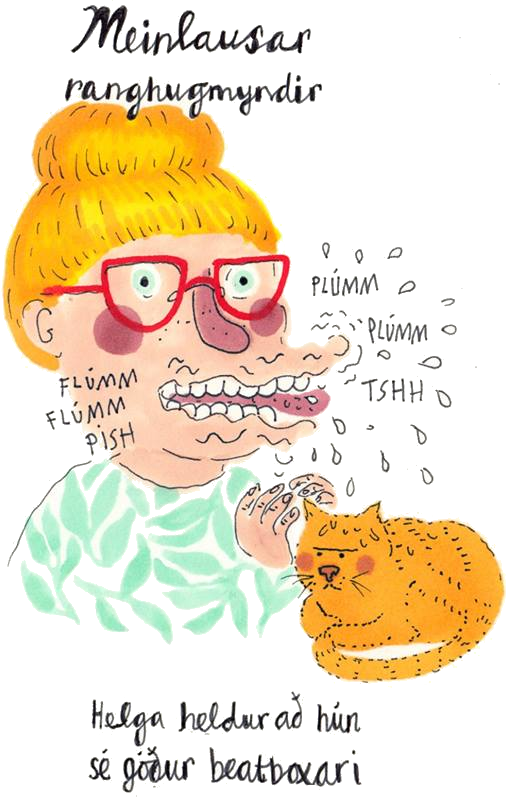
\includegraphics[width=\textwidth]{figures/helga}
                \vfill
                by L\'{o}aborator\'{i}um
            \end{column}
        \end{columns}
    \end{frame}

    \begin{frame}
        \frametitle{About ICECATS}
        \begin{columns}[T]
            \begin{column}{0.55\textwidth}
                \begin{itemize}
                    \item A literary and feline entertainment podcast*
                    \item Discuss the erotic and surreal book series The Legend of the Ice People by Margit Sandemo
                    \item Each episode covers part of a book from the series, providing listeners a journey through
                    \item Margit's
                    world of witches, demons, and powerful women
                    \item Each episode concludes with a segment on cats, exploring cat history and significant
                    cats through the ages
                \end{itemize}
            \end{column}
            \begin{column}{0.45\textwidth}
                \centering
                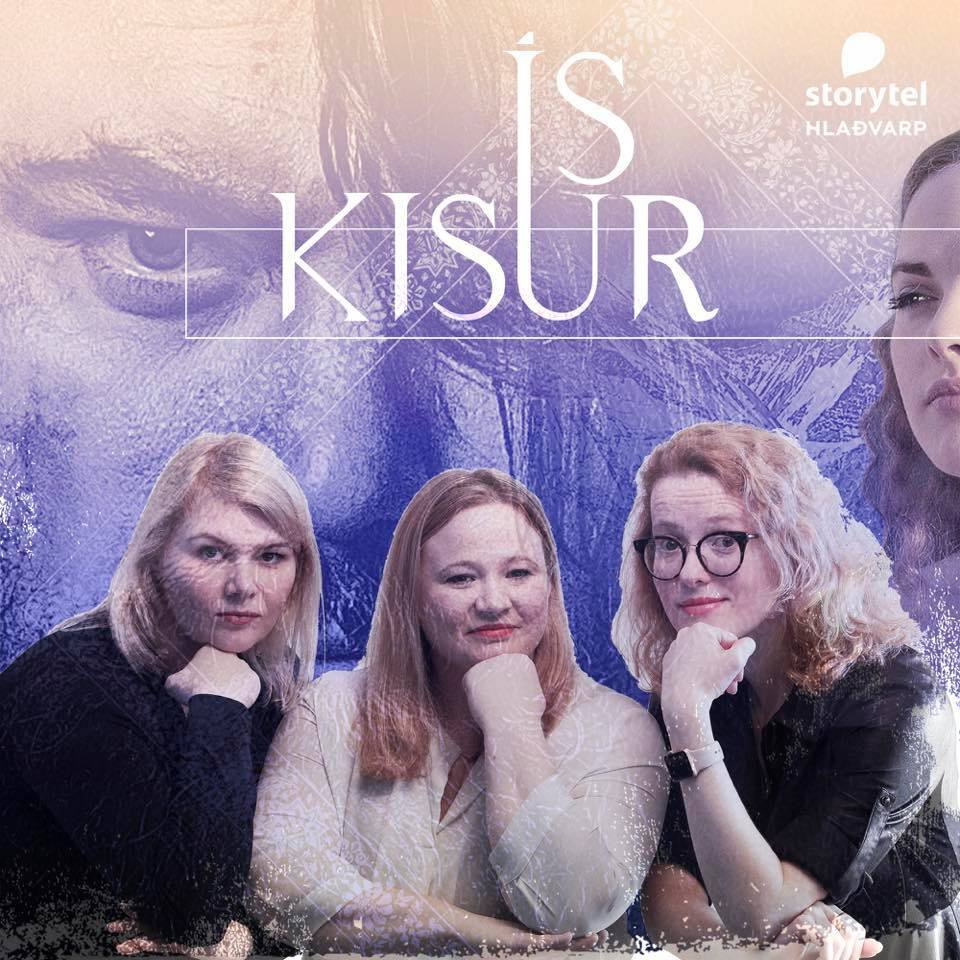
\includegraphics[width=\textwidth]{figures/podcast_image.jpg}
                \vfill
                Birna, Krist\'{i}n, and dr.~Helga\\
                \vspace{12pt}
                \footnotesize{*\emph{None of the hosts are actually cats or literary experts.}}
            \end{column}
        \end{columns}
    \end{frame}

    \begin{frame}
        \frametitle{Margit Sandemo, 1924-2018}
        \begin{columns}[T]
            \begin{column}{0.55\textwidth}
                \begin{itemize}
                    \item Father was a Norwegian poet, Anders Underdal
                    \item Claimed lineage to Nobel Prize-winning author Bjornstjerne Bjornson
                    \item First published at forty years old
                    \item Best-selling author in the Nordic countries since the 1980s
                    \item Most notable book series:
                    \begin{itemize}
                        \item \emph{The Legend of the Ice People} 1982-89 (\#47)
                        \item \emph{The Warlock} 1991-94 (\#15)
                        \item \emph{The Legend of the Realm of Light} 1995-99 (\#12)
                    \end{itemize}
                \end{itemize}
            \end{column}
            \begin{column}{0.45\textwidth}
                \centering
                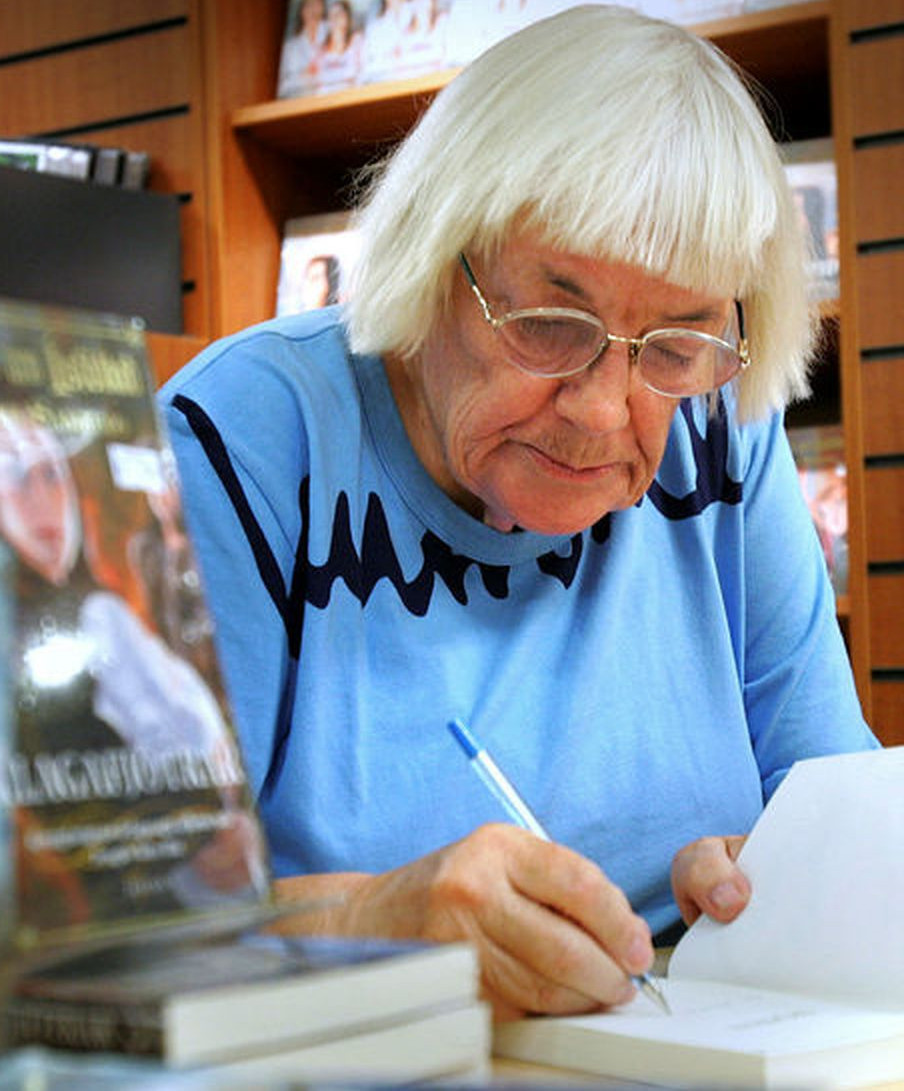
\includegraphics[width=\textwidth]{figures/margit_sandemo}
            \end{column}
        \end{columns}
    \end{frame}

    \begin{frame}
        \frametitle{Publications}
        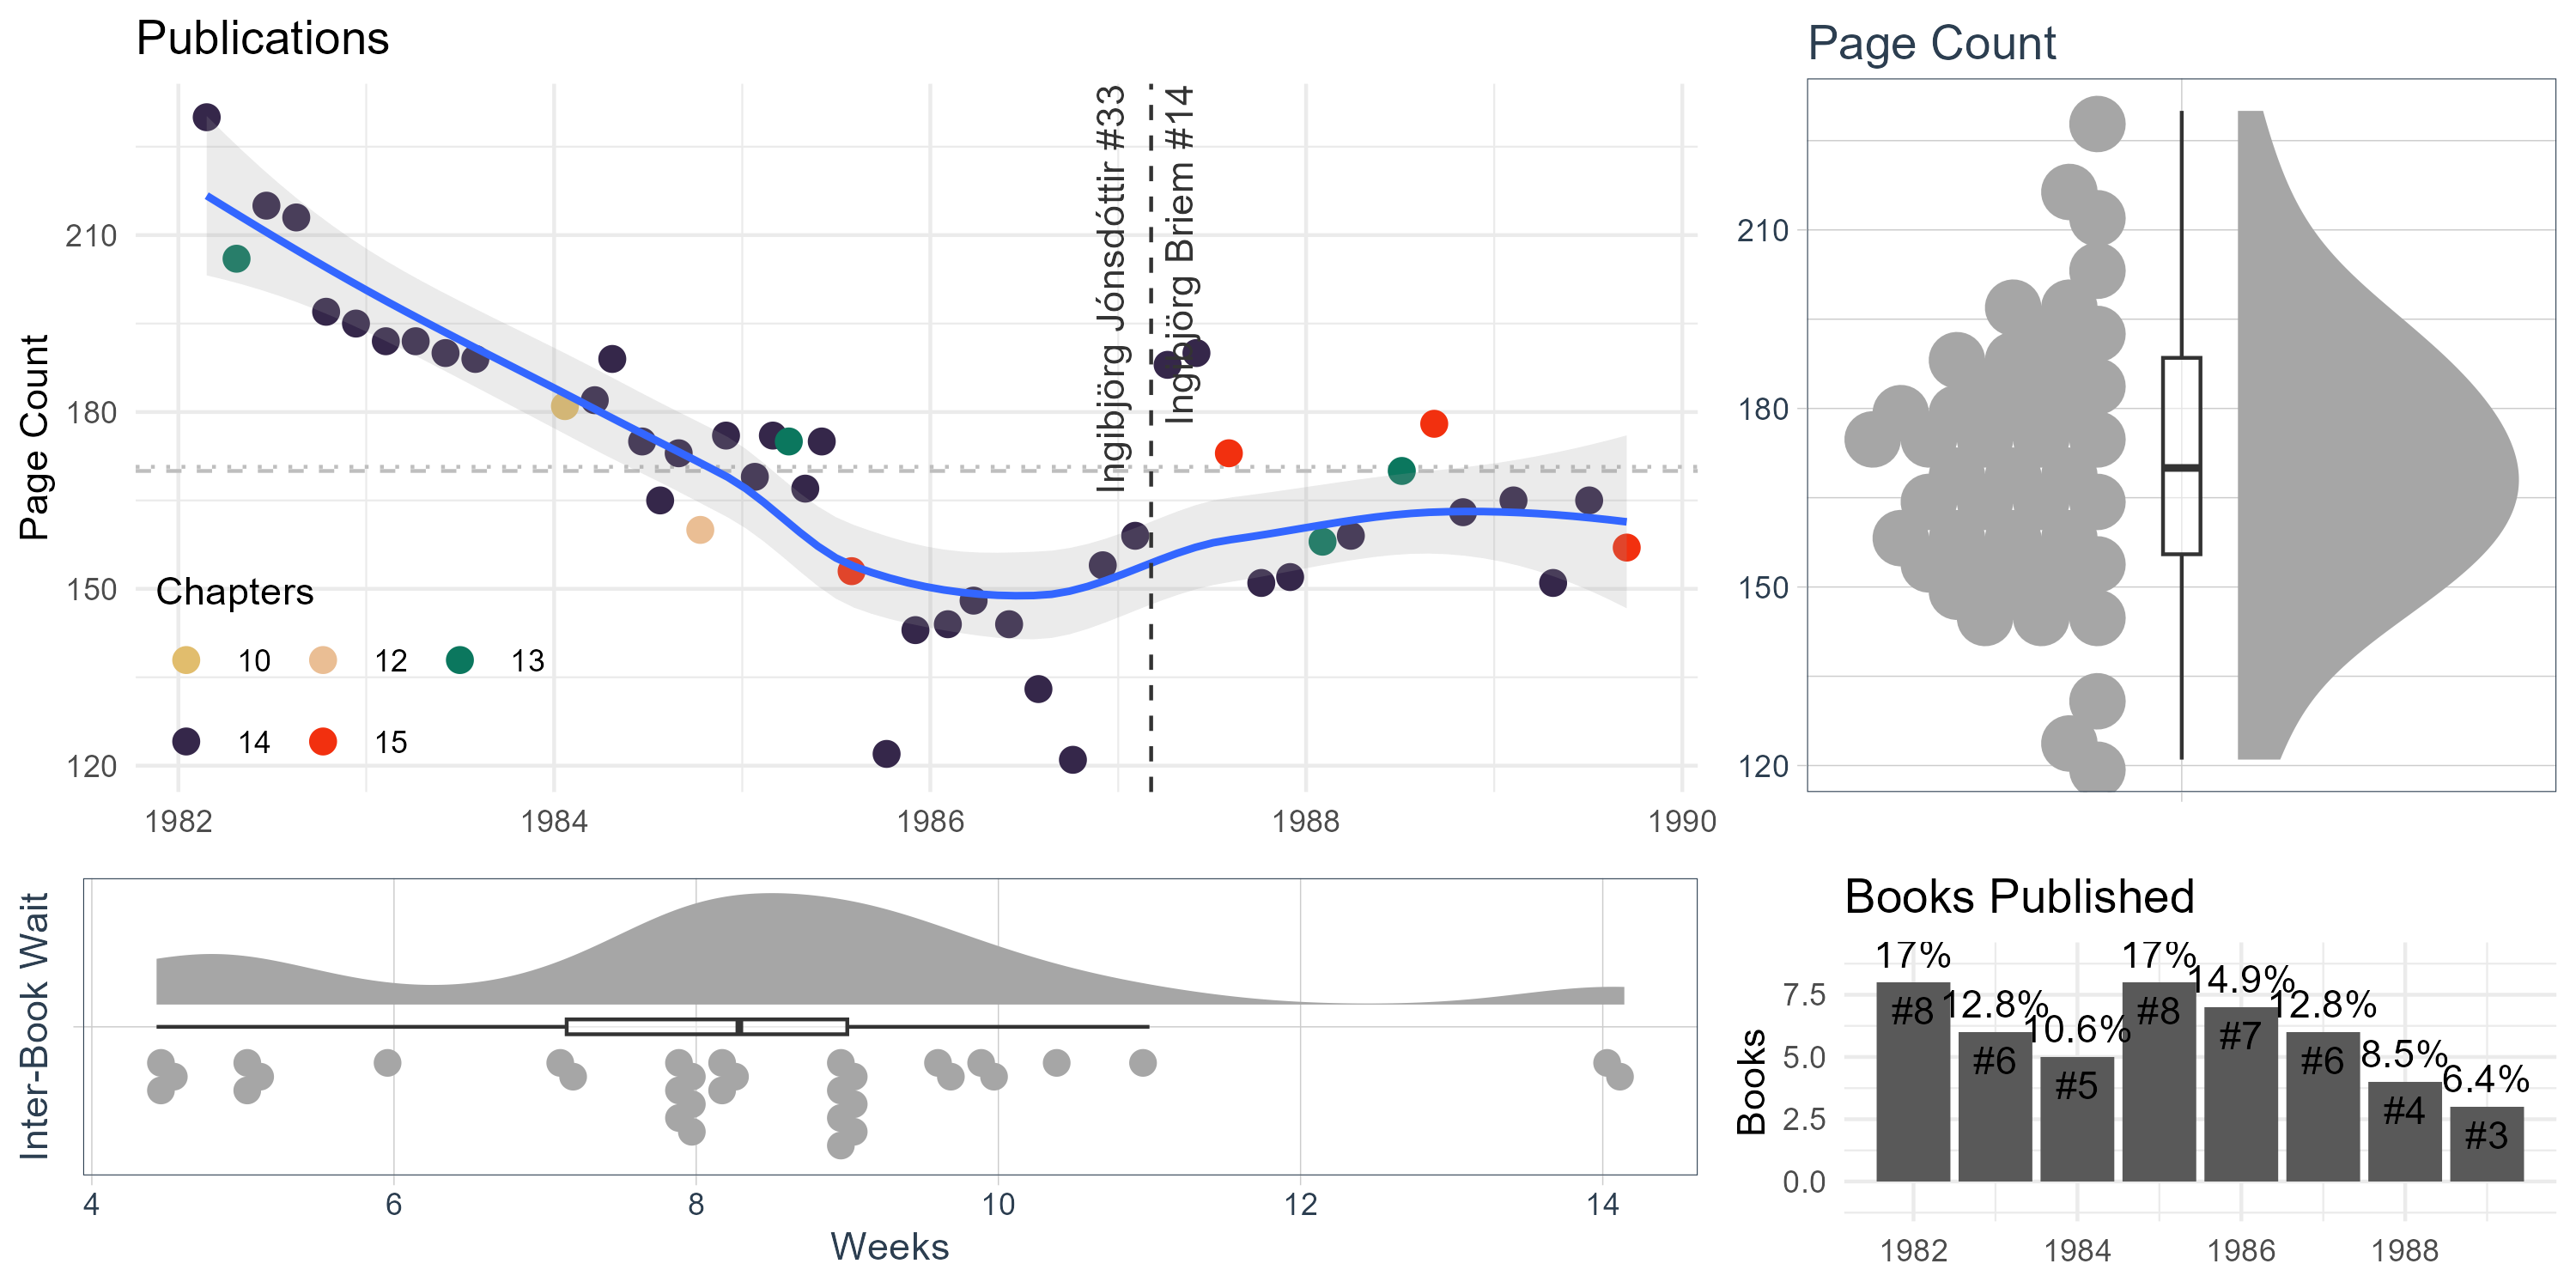
\includegraphics[width=\textwidth]{charts/margit_count}
        \vspace{-24pt}
        \begin{itemize}
            \item 47 books, 652 chapters, 8023 pages, 8 years
            \item Average book length: 170 pages (avg. 13.9 chapters)
            \item Released at a rate of 1 book every 2 months (avg. 57.9 days), usually on Tuesdays
        \end{itemize}
    \end{frame}

    \begin{frame}
        \frametitle{Audiobooks on Storytel: Active Fanbase}
        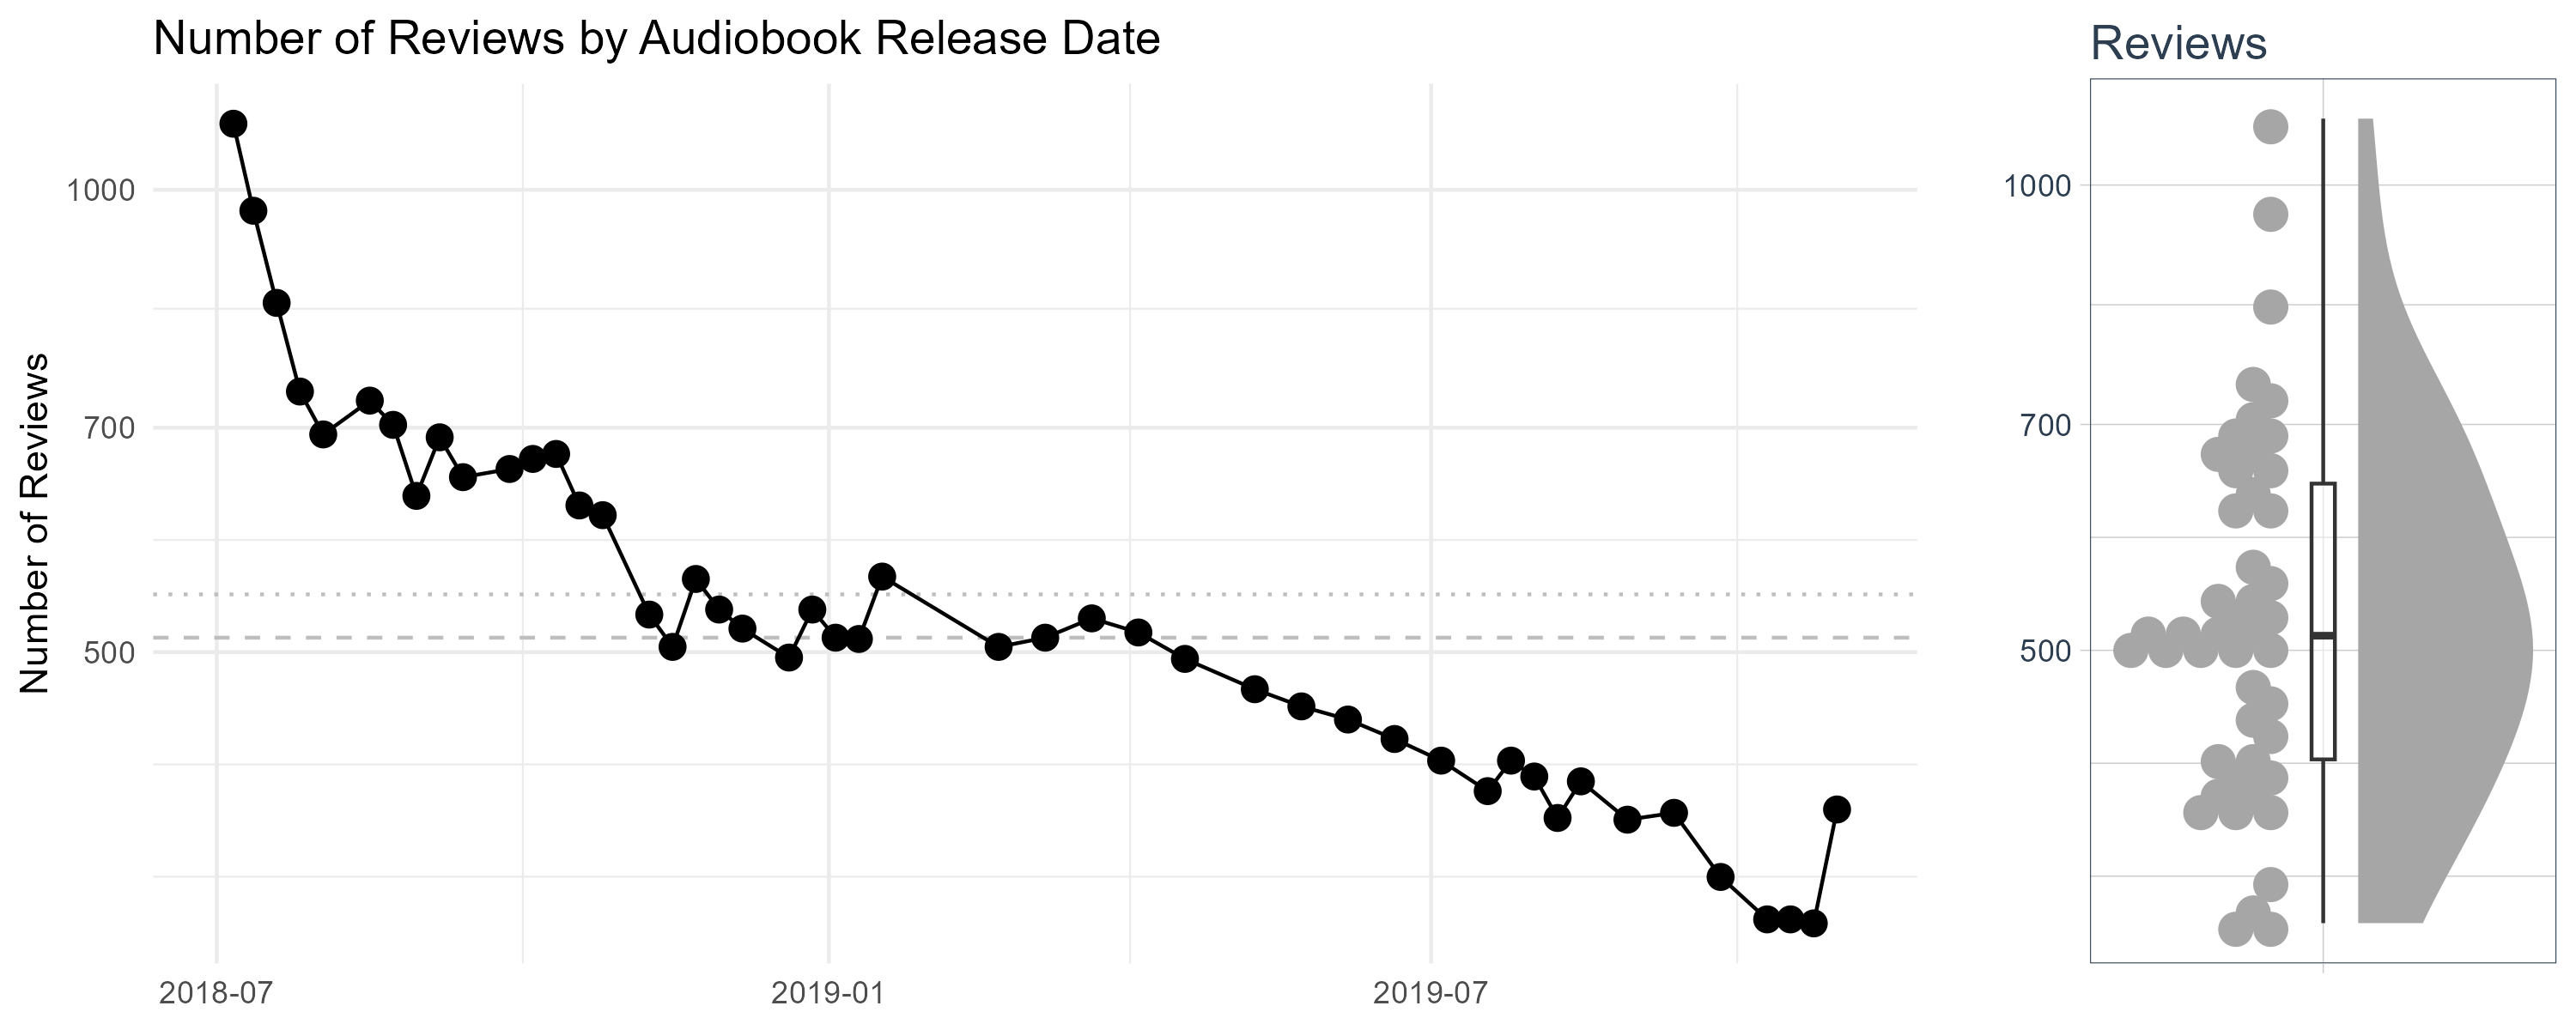
\includegraphics[width=\textwidth]{charts/storytel_reviews}

        The series has a dedicated fanbase, with consistently high engagement, a solid median review count of 511,
        and even the least-reviewed book gathering 333 reviews.

        Releases on Thursdays, spaced 1--2 weeks apart, over 16-months.

    \end{frame}

    \begin{frame}
        \frametitle{Audiobooks on Storytel: High Ratings}
        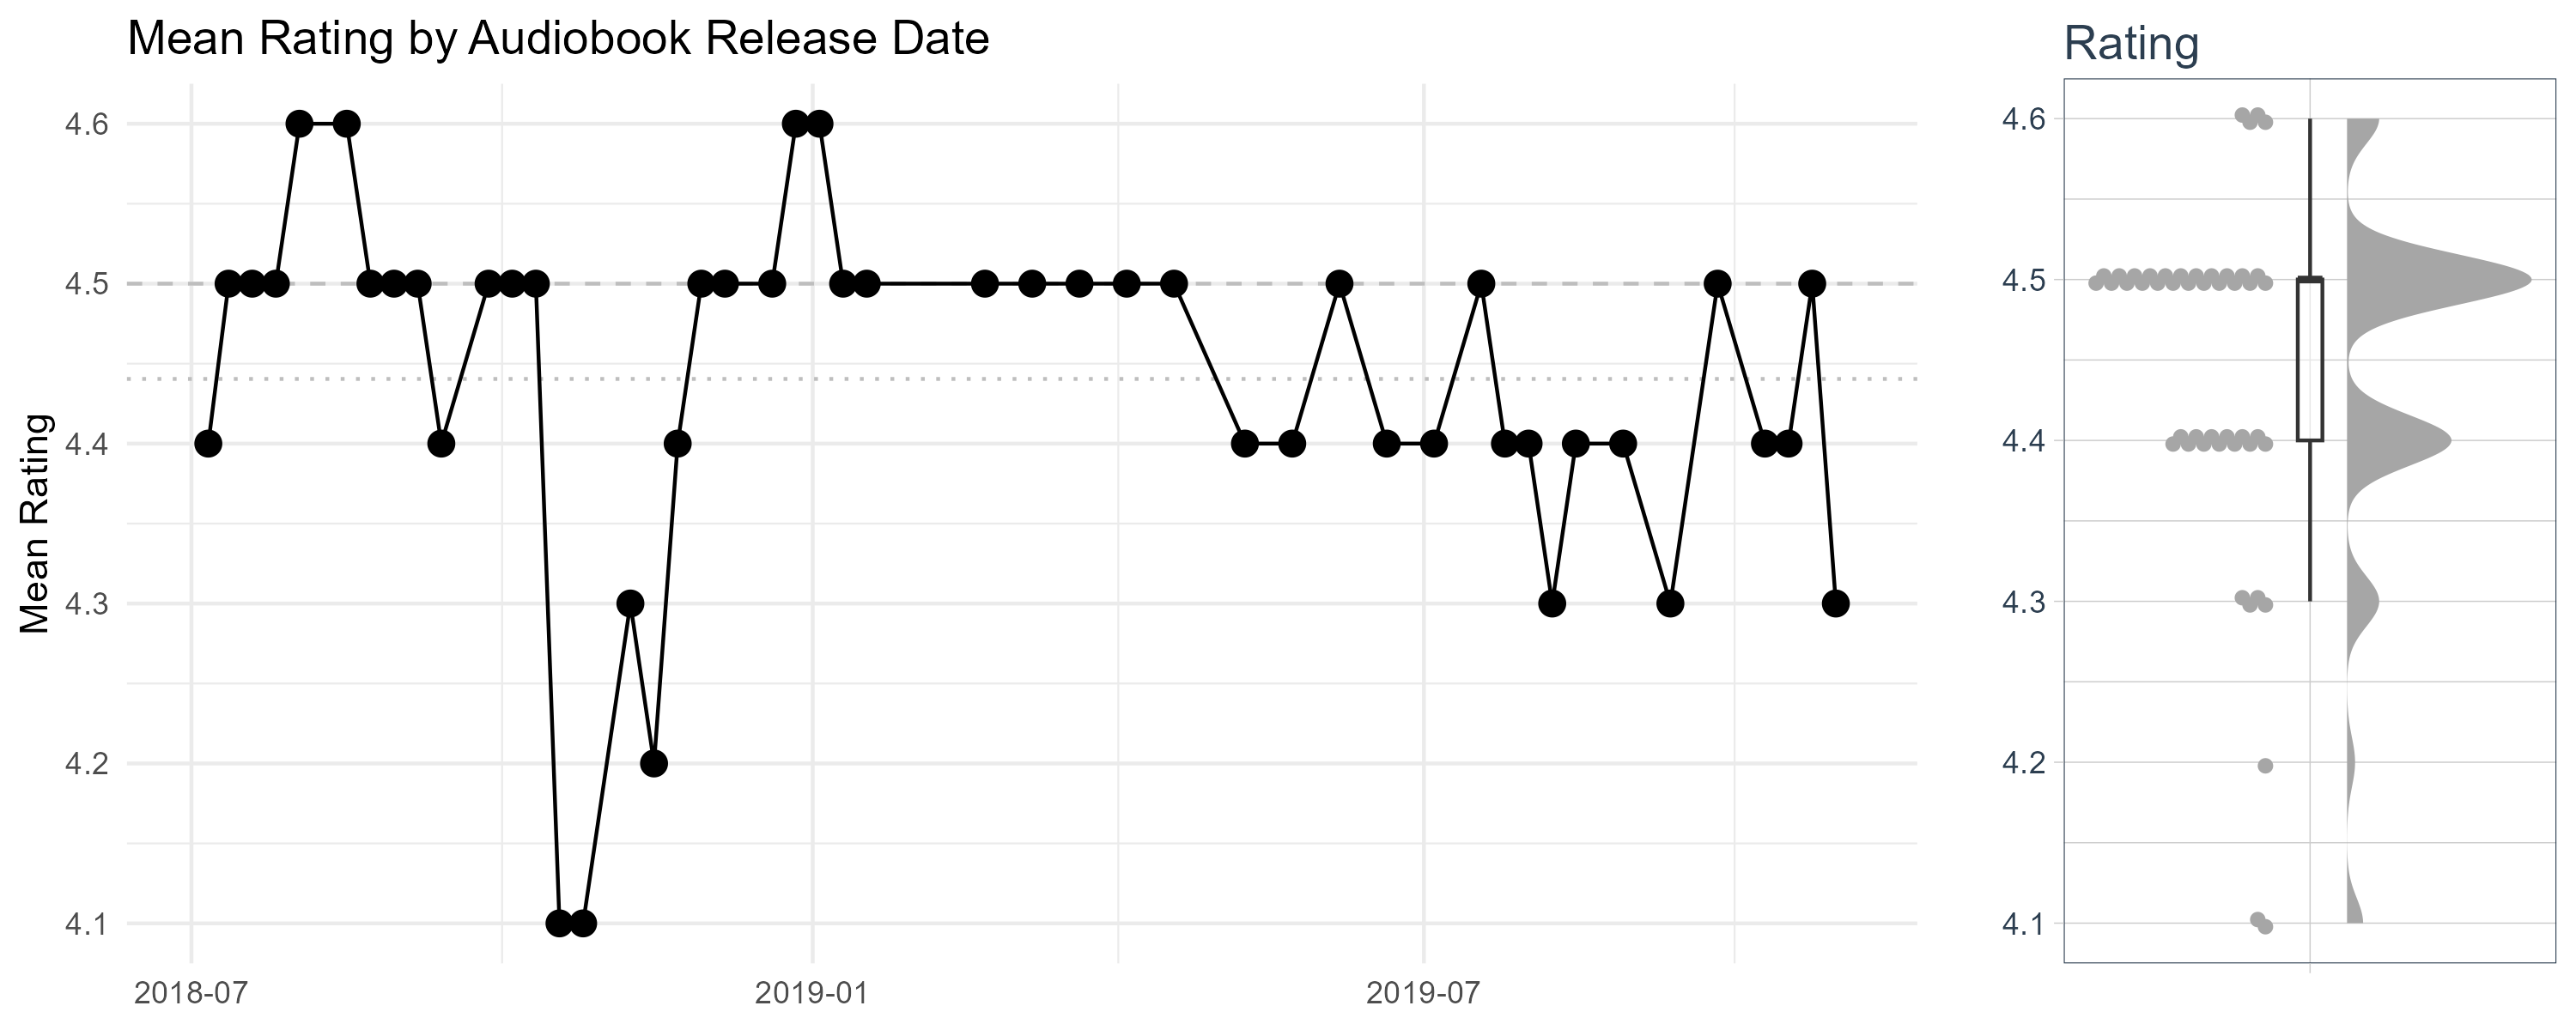
\includegraphics[width=\textwidth]{charts/storytel_ratings}

        Despite a few lower outliers, which can be attributed to a lack of resonance with certain readers and the
        repetitive and slower pace towards the end of the series, the overall rating remains high, with an average
        4.44 stars out of 5.


    \end{frame}

    \begin{frame}
        \frametitle{Audiobooks on Storytel: Our Narrators}
        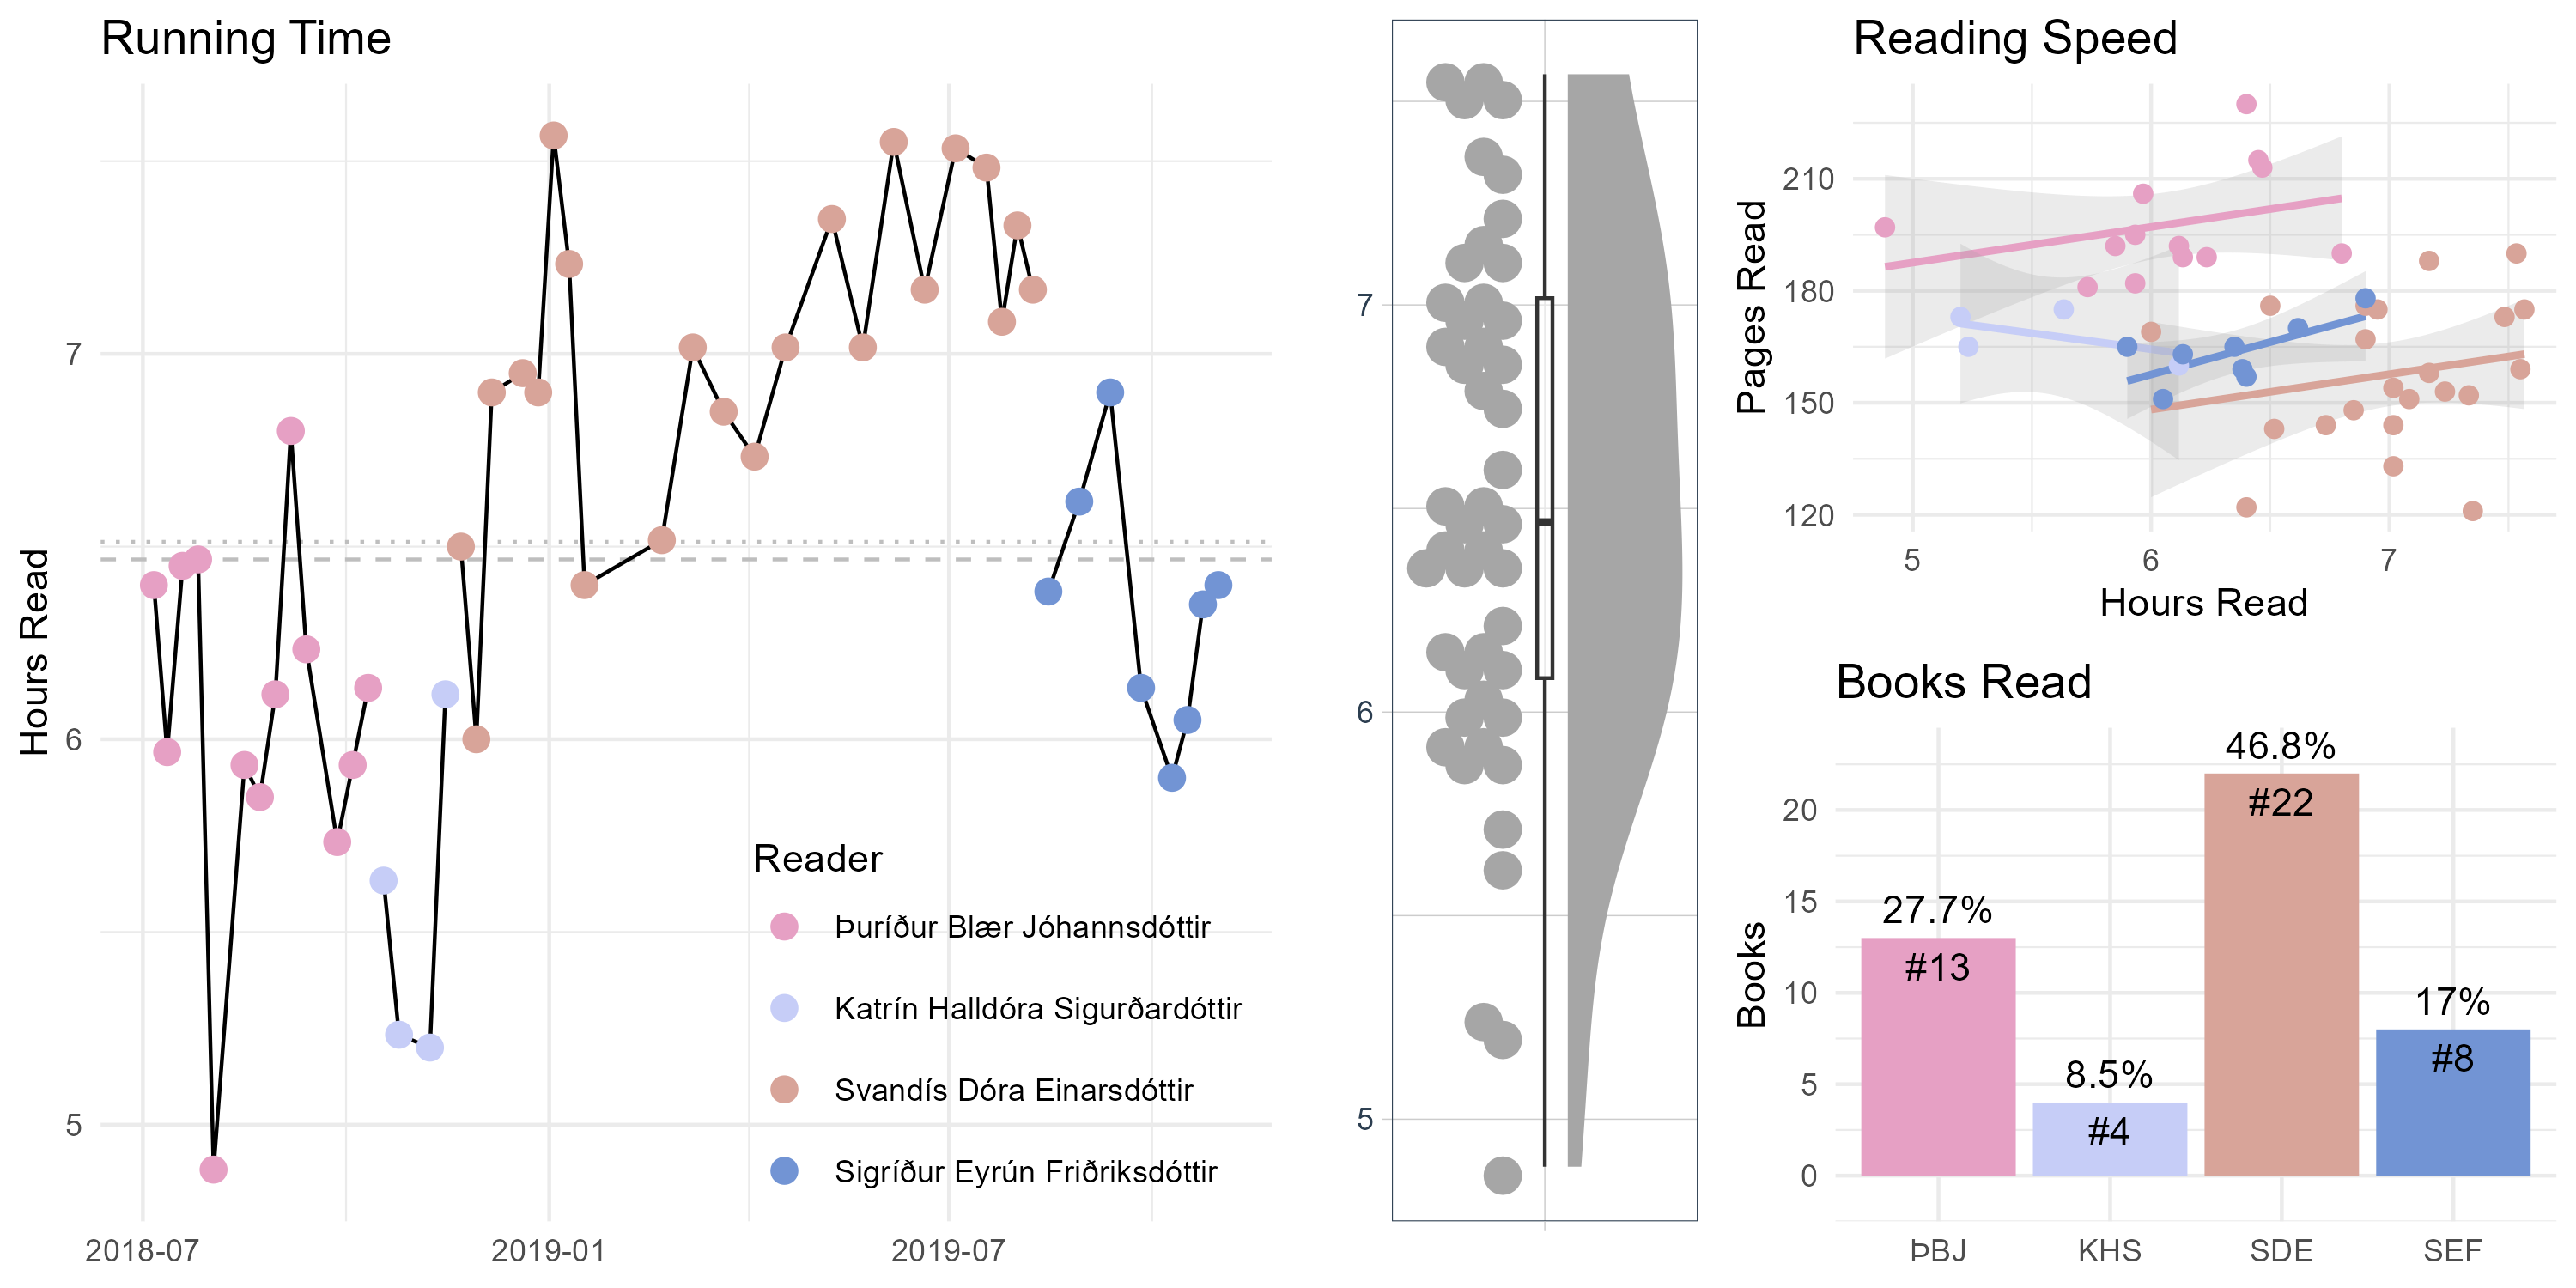
\includegraphics[width=\textwidth]{charts/storytel_readers}
        \vspace{-18pt}
        \begin{itemize}
            \item Over 18K minutes of romantic medieval fantasy -- 12.8 days of continuous listening
            \item Four distinct voices with varied reading styles and perseverance with the series
        \end{itemize}
    \end{frame}

    \begin{frame}
        \frametitle{ICECATS Podcast Timeline}

        \textbf{Alvarpi\dh{} Era:}
        \begin{itemize}
            \item Syndicated on the Icelandic podcast platform Alvarpi\dh{} on the news site N\'{u}t\'{i}minn.
            \item Debut on February 23\textsuperscript{rd} 2017 (Alvarpi\dh's 3\textsuperscript{rd} birthday).
            \item Shared the platform with other renowned podcasts like \emph{Hefnendur} and \emph{Englaryk}.
            \item Last aired on November 1\textsuperscript{st} 2018, after 46 episodes.
        \end{itemize}

        \textbf{Storytel Era:}
        \begin{itemize}
            \item Syndicated on the Icelandic audiobook platform Storytel.
            \item First of three podcasts ever featured on the platform
            (with \emph{Skr\ae{}\dh{}ur} and \emph{Seg\dh{}u m\'{e}r s\"{o}gu})
            \item Debut March 7\textsuperscript{th} 2019, and completed after 96 episodes on December 17\textsuperscript{th}, 2020.
        \end{itemize}

    \end{frame}


    \begin{frame}
        \frametitle{Podcast on Alvarpi\dh{}: Listenership on \url{nutiminn.is}}
        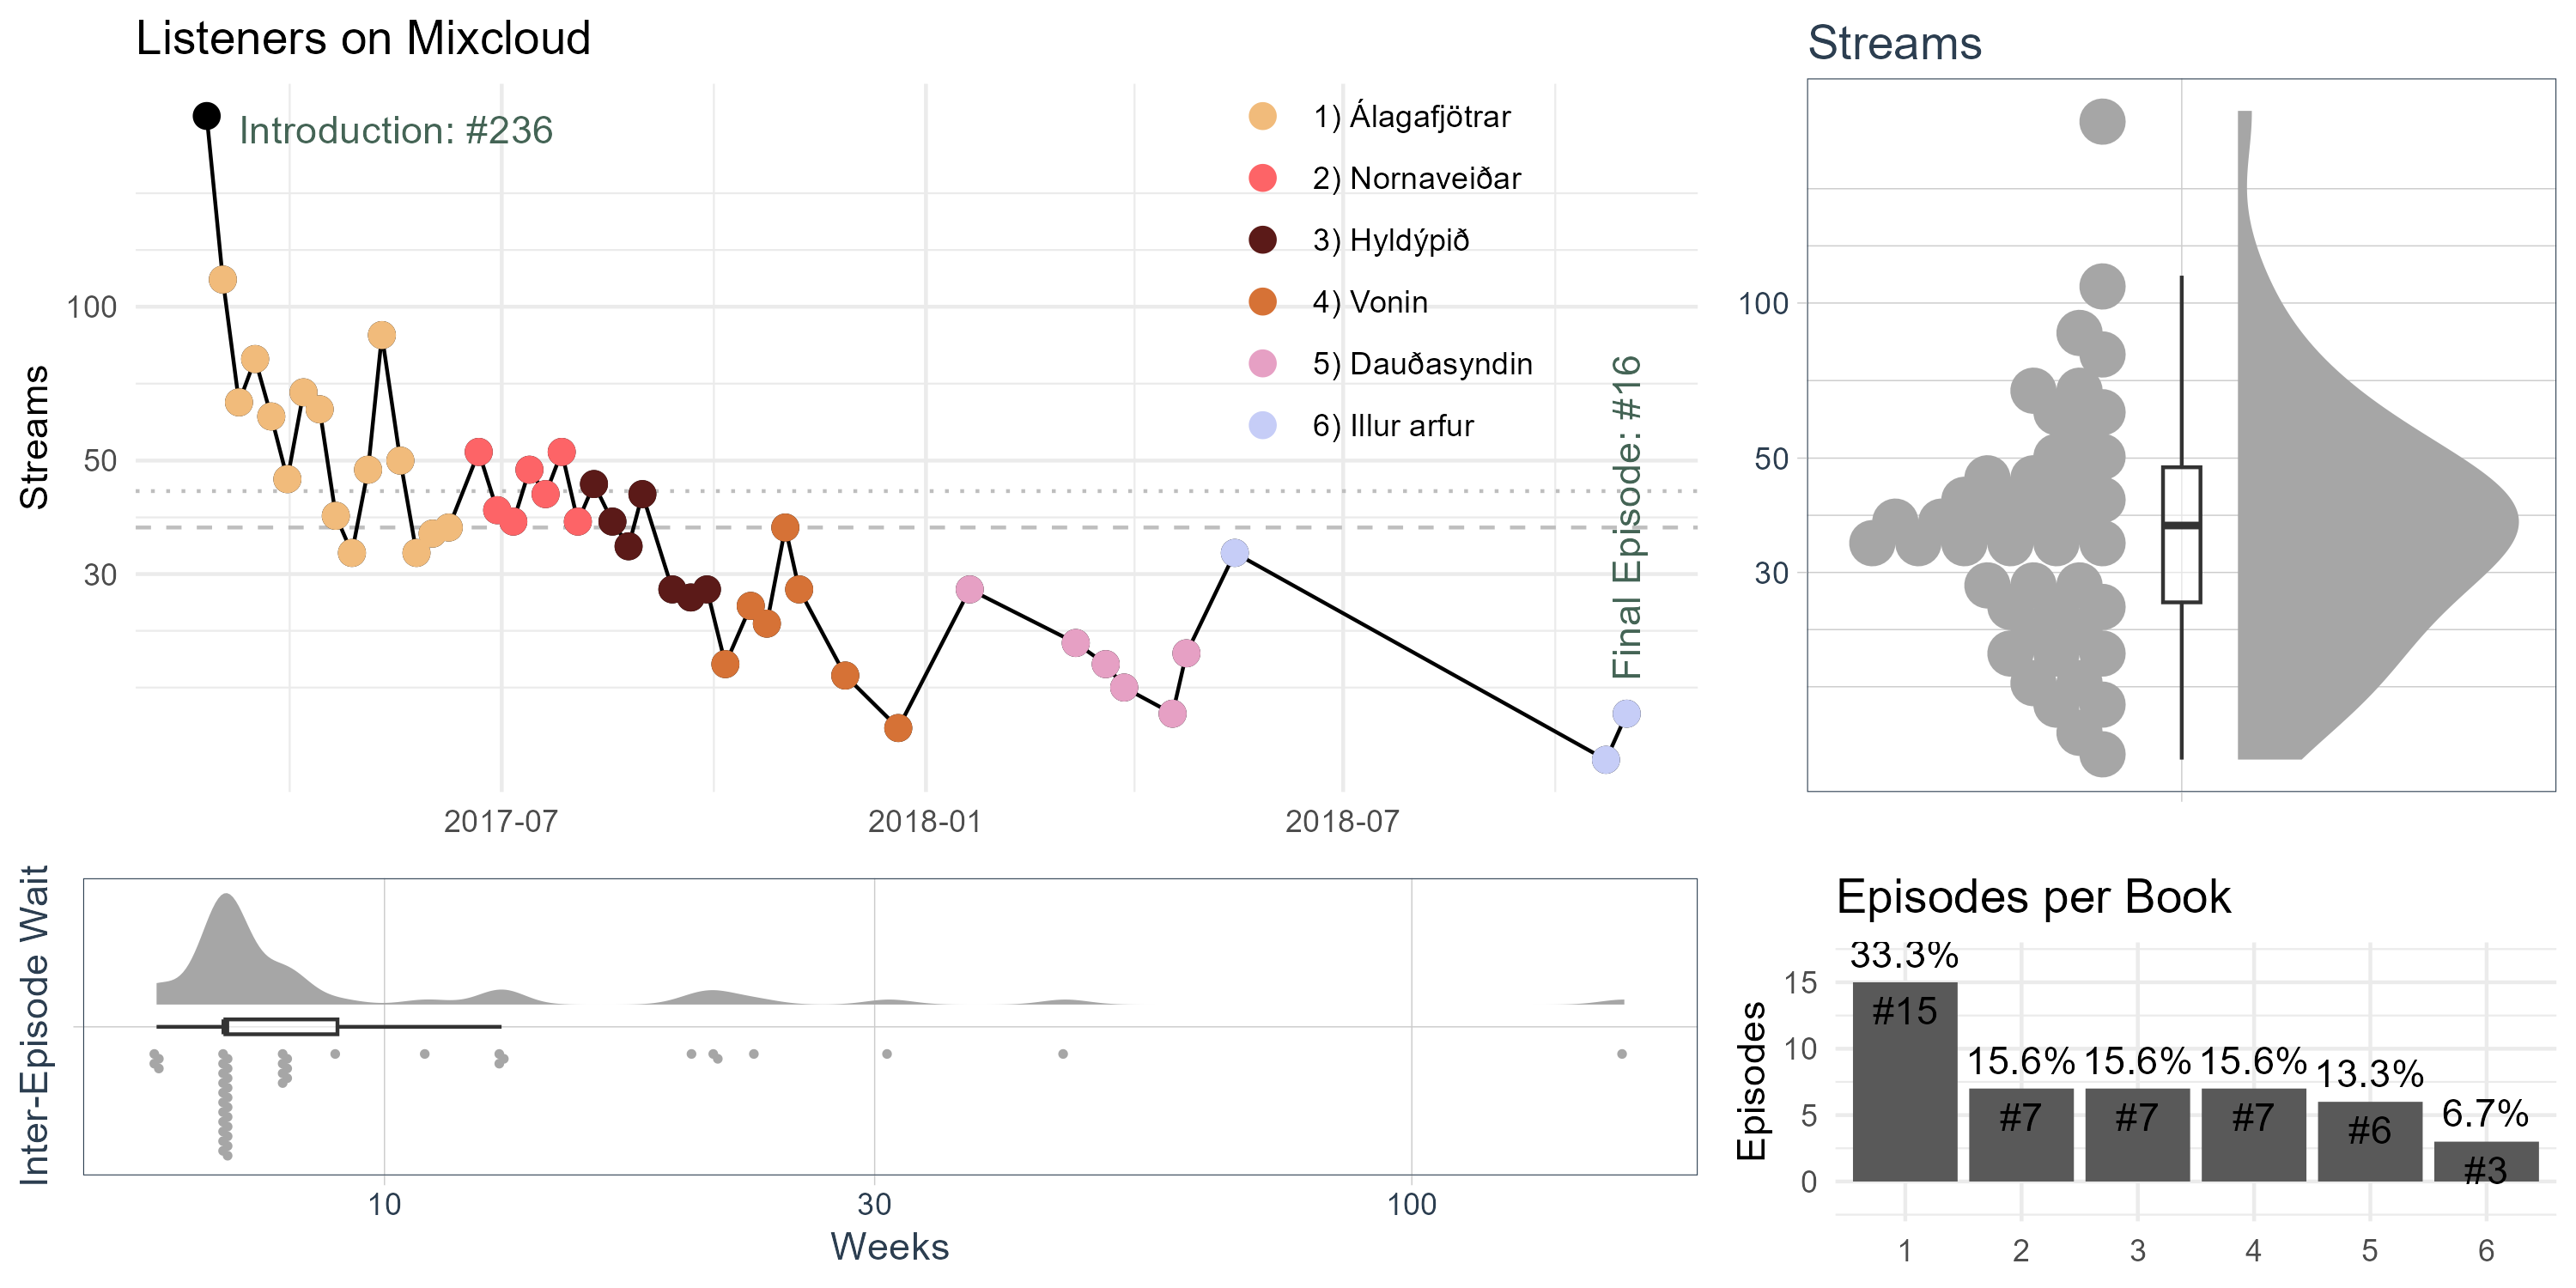
\includegraphics[width=\textwidth]{charts/alvarpid_listeners.png}

        \begin{itemize}
            \item 46 episodes, 20 months, 5.5 books
            \item 2231 minutes -- 37 hours -- 1.5 days of continuous listening
            \item Roughly 1040 streams per episode (thereof ~40 in browser)
        \end{itemize}

    \end{frame}


    \begin{frame}
        \frametitle{Podcast on Storytel: Hours Rambled}
        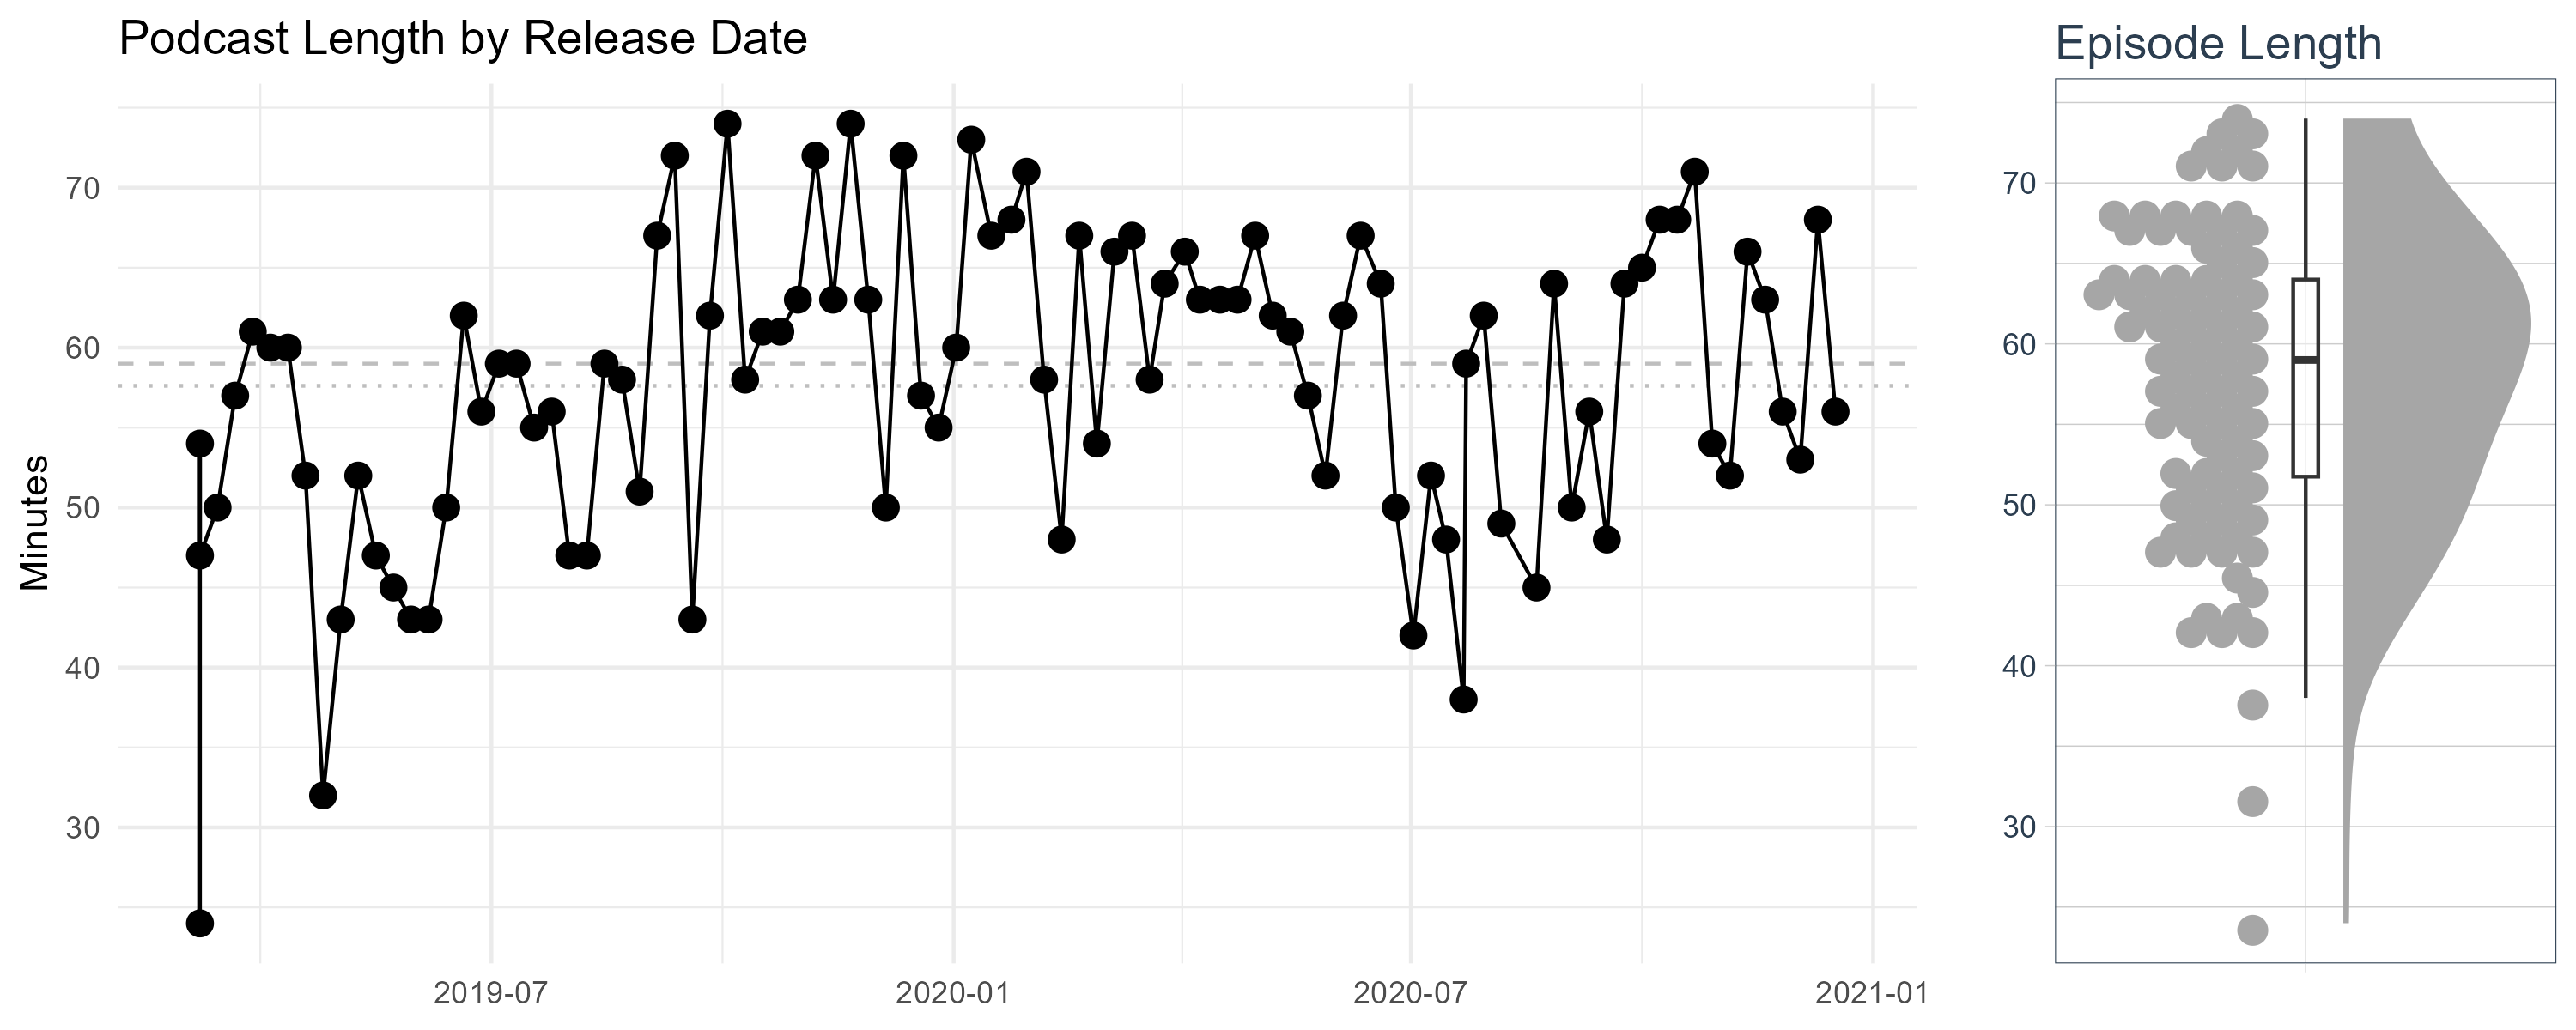
\includegraphics[width=\textwidth]{charts/iskisur_length}

        Over a period of 21 months, there is 5531 minutes of \emph{quality} content, or 3.8 days of continuous
        listening.

        Median length is 59 minutes, but never surpassing 75 minutes.

    \end{frame}

    \begin{frame}
        \frametitle{Podcast on Storytel: High Ratings}
        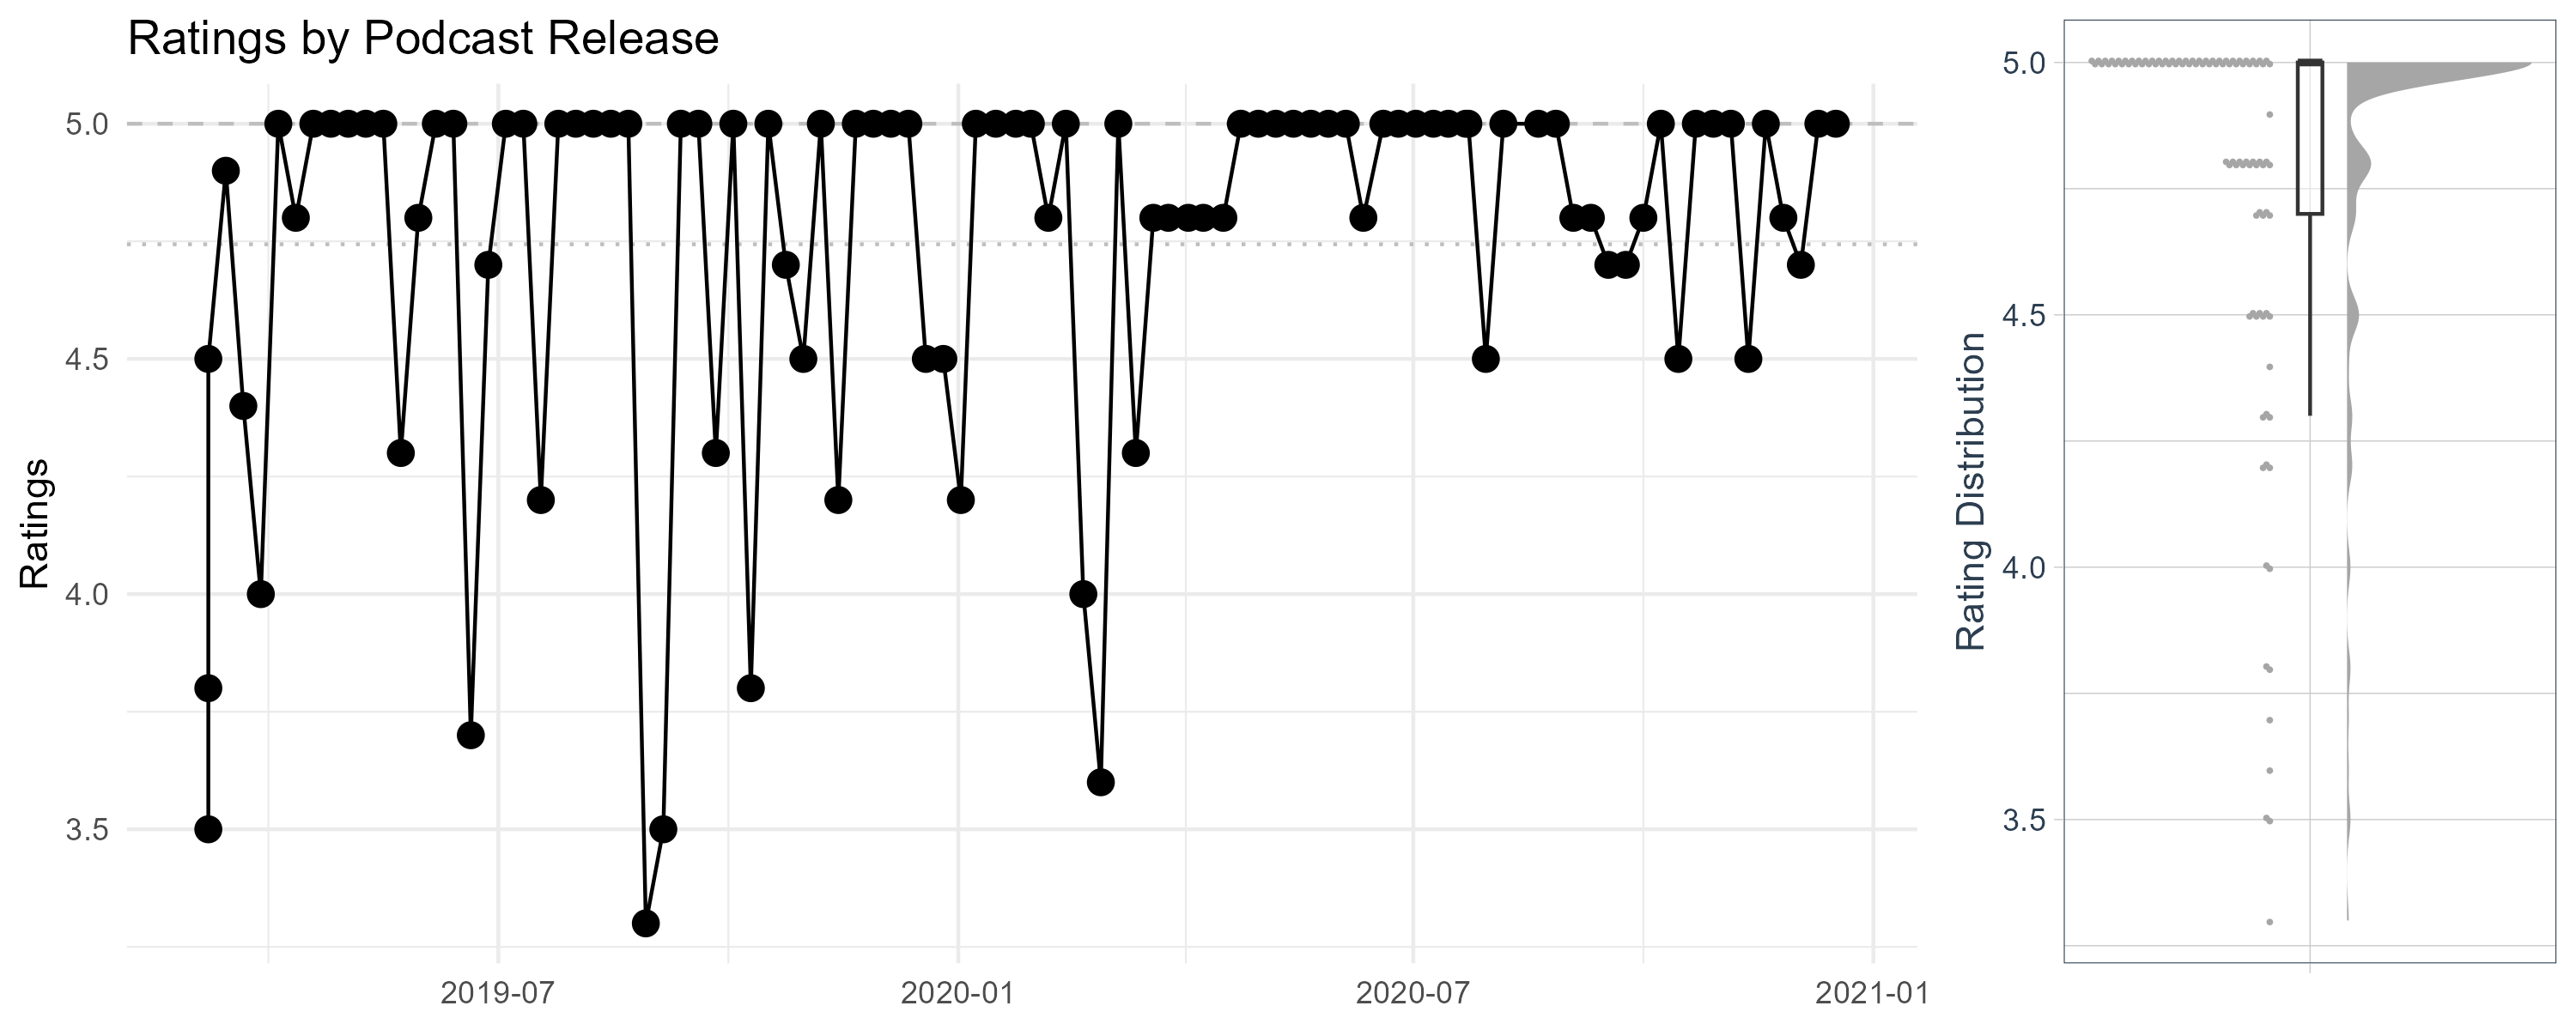
\includegraphics[width=\textwidth]{charts/iskisur_ratings}
        \begin{itemize}
            \item Average rating: 4.74 out of 5
            \item 54 episodes with a perfect 5.0 score (56\% of total)
            \item Only 4 episodes with a rating below 4.0 (worst case 3.3)
        \end{itemize}
    \end{frame}

    \begin{frame}
        \frametitle{Podcast on Storytel: Low Reviews}
        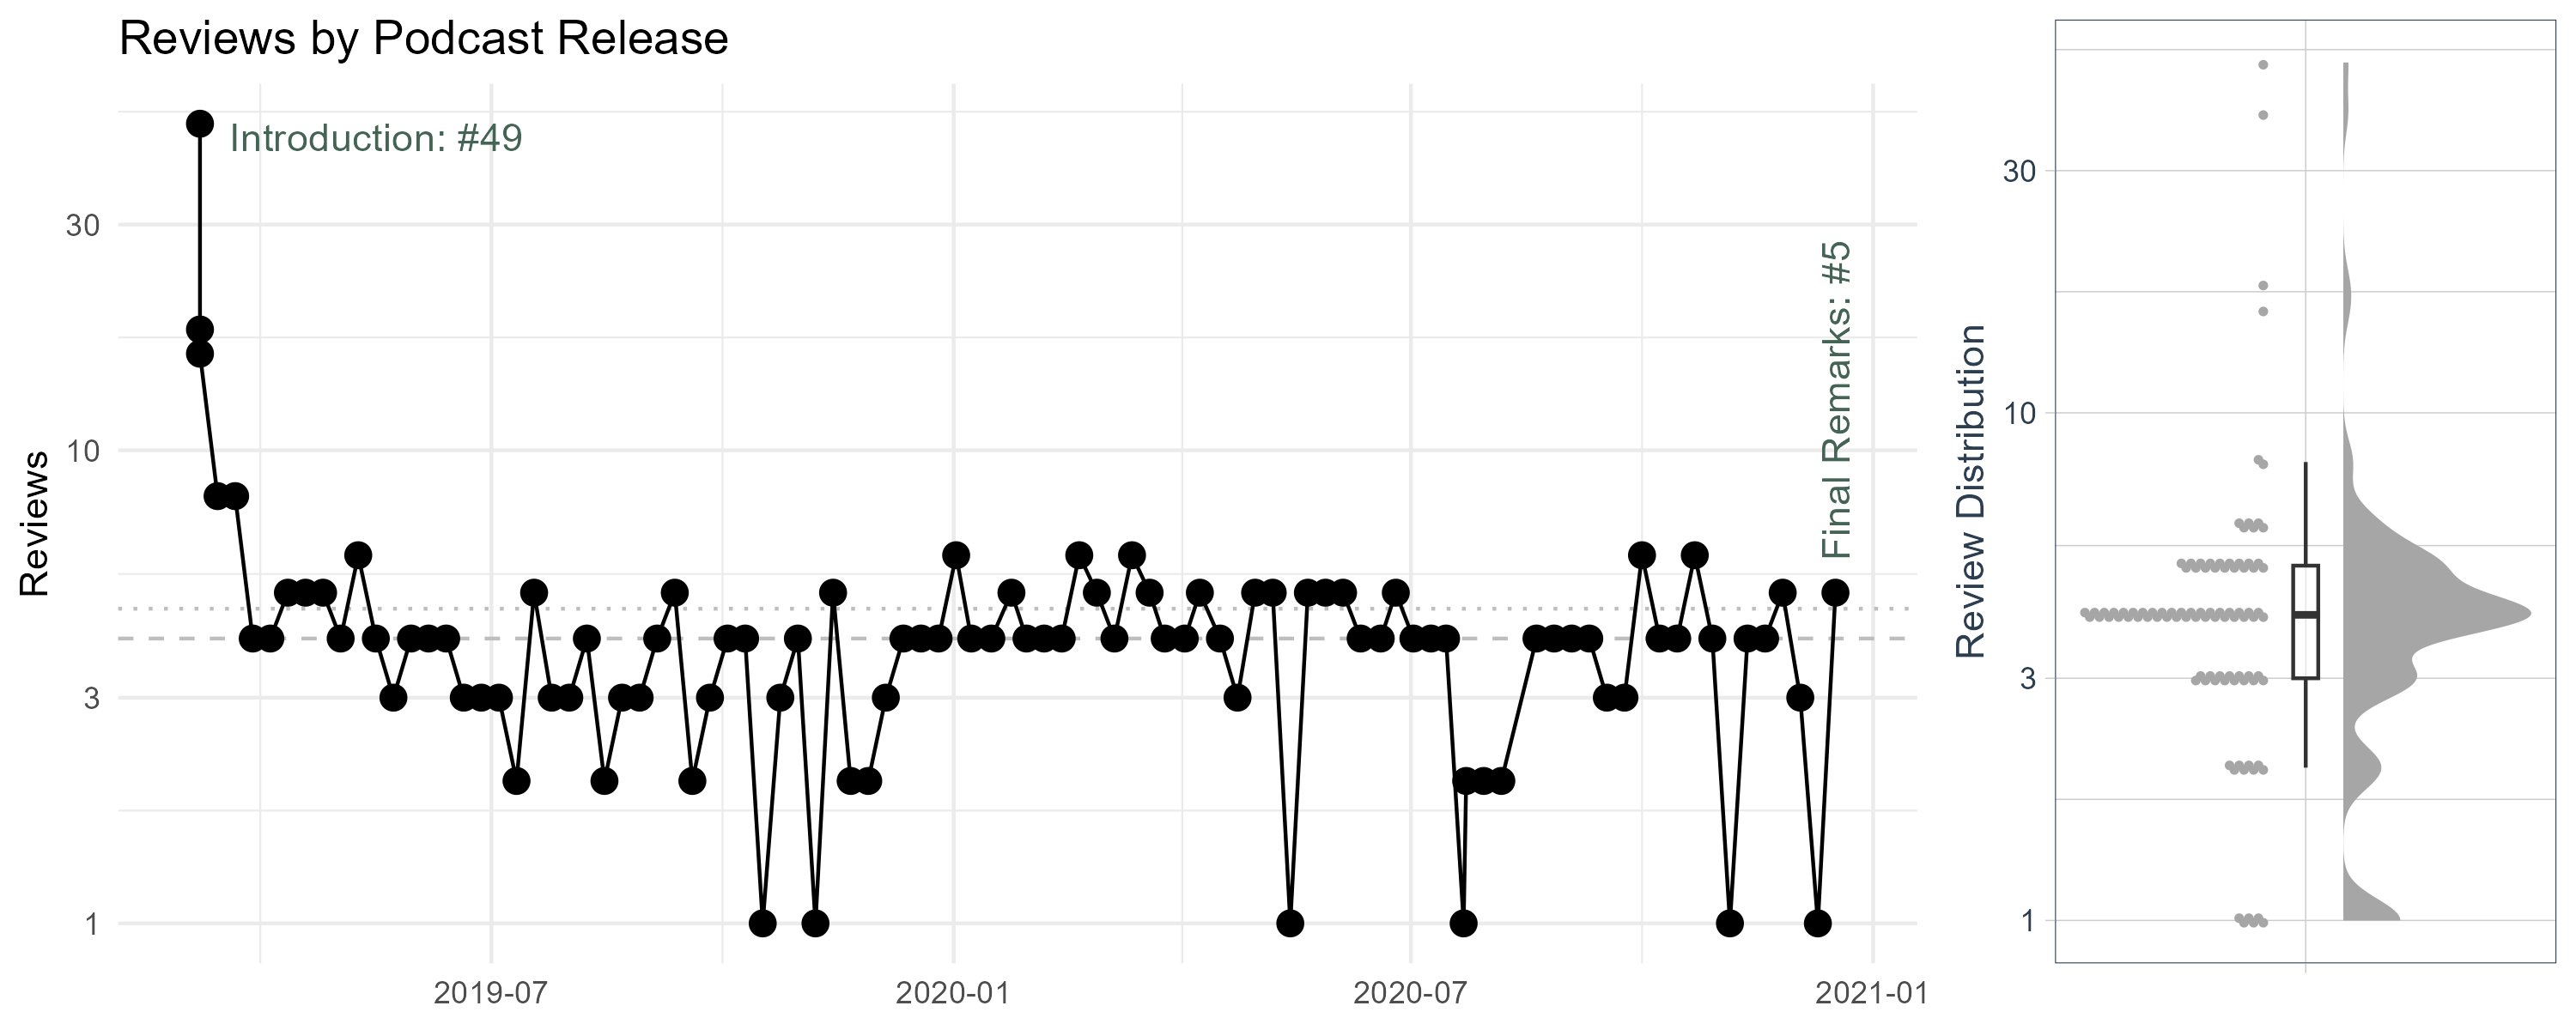
\includegraphics[width=\textwidth]{charts/iskisur_reviews}

        \begin{itemize}
            \item Number of reviews: 444 total (25,627 for the audiobooks)
            \item At least one active fan throughout the period
            \item Four regular fans who consistently provided review
        \end{itemize}

        %Please note that while the high ratings may seem impressive, we humbly acknowledge that they might not be
        %entirely trustworthy. The number of reviews for the podcast, 444 in total, pales in comparison to the 25,
        %627 reviews received for the audio books. Nevertheless, we are grateful for the 49 reviews received for
        %the inaugural introduction episode, and we appreciate the dedication of at least one active fan
        %throughout the podcast's duration. Additionally, we extend our heartfelt thanks to the four regular fans
        %who consistently supported us by providing reviews.

    \end{frame}

    \begin{frame}
        \frametitle{Podcast Platform Comparison}

        \begin{table}[]
            \begin{tabular}{l|rr|rr|rrr|r}
                & \rotatebox{90}{Episodes} & \rotatebox{90}{Books} &
                \rotatebox{90}{Total Running Time (hours)} & \rotatebox{90}{Average Length (min)} &
                \rotatebox{90}{Median Days to Next}
                & \rotatebox{90}{Average Days to Next}  & \rotatebox{90}{Max Days to Next}  &
                \rotatebox{90}{Months Active} \\
                \midrule
                Alvarpi\dh   & 46  & 6 & 37.2  & 48.50 & 7 & 13.69  & 161  & 20.3  \\
                Storytel           & 96 & 47    & 92.2 & 57.61       & 7   & 6.85       & 14     & 21.4 \\
                \midrule
                & 142 &    & 129.4 &       &   &       &     & 45.8*
            \end{tabular}
        \end{table}

        \vfill
        \footnotesize{*4.1 months hiatus between Alvarpi\dh{} and Storytel}
    \end{frame}

    \begin{frame}
        \frametitle{Timeline for the Legend of the Ice Cat-People}
        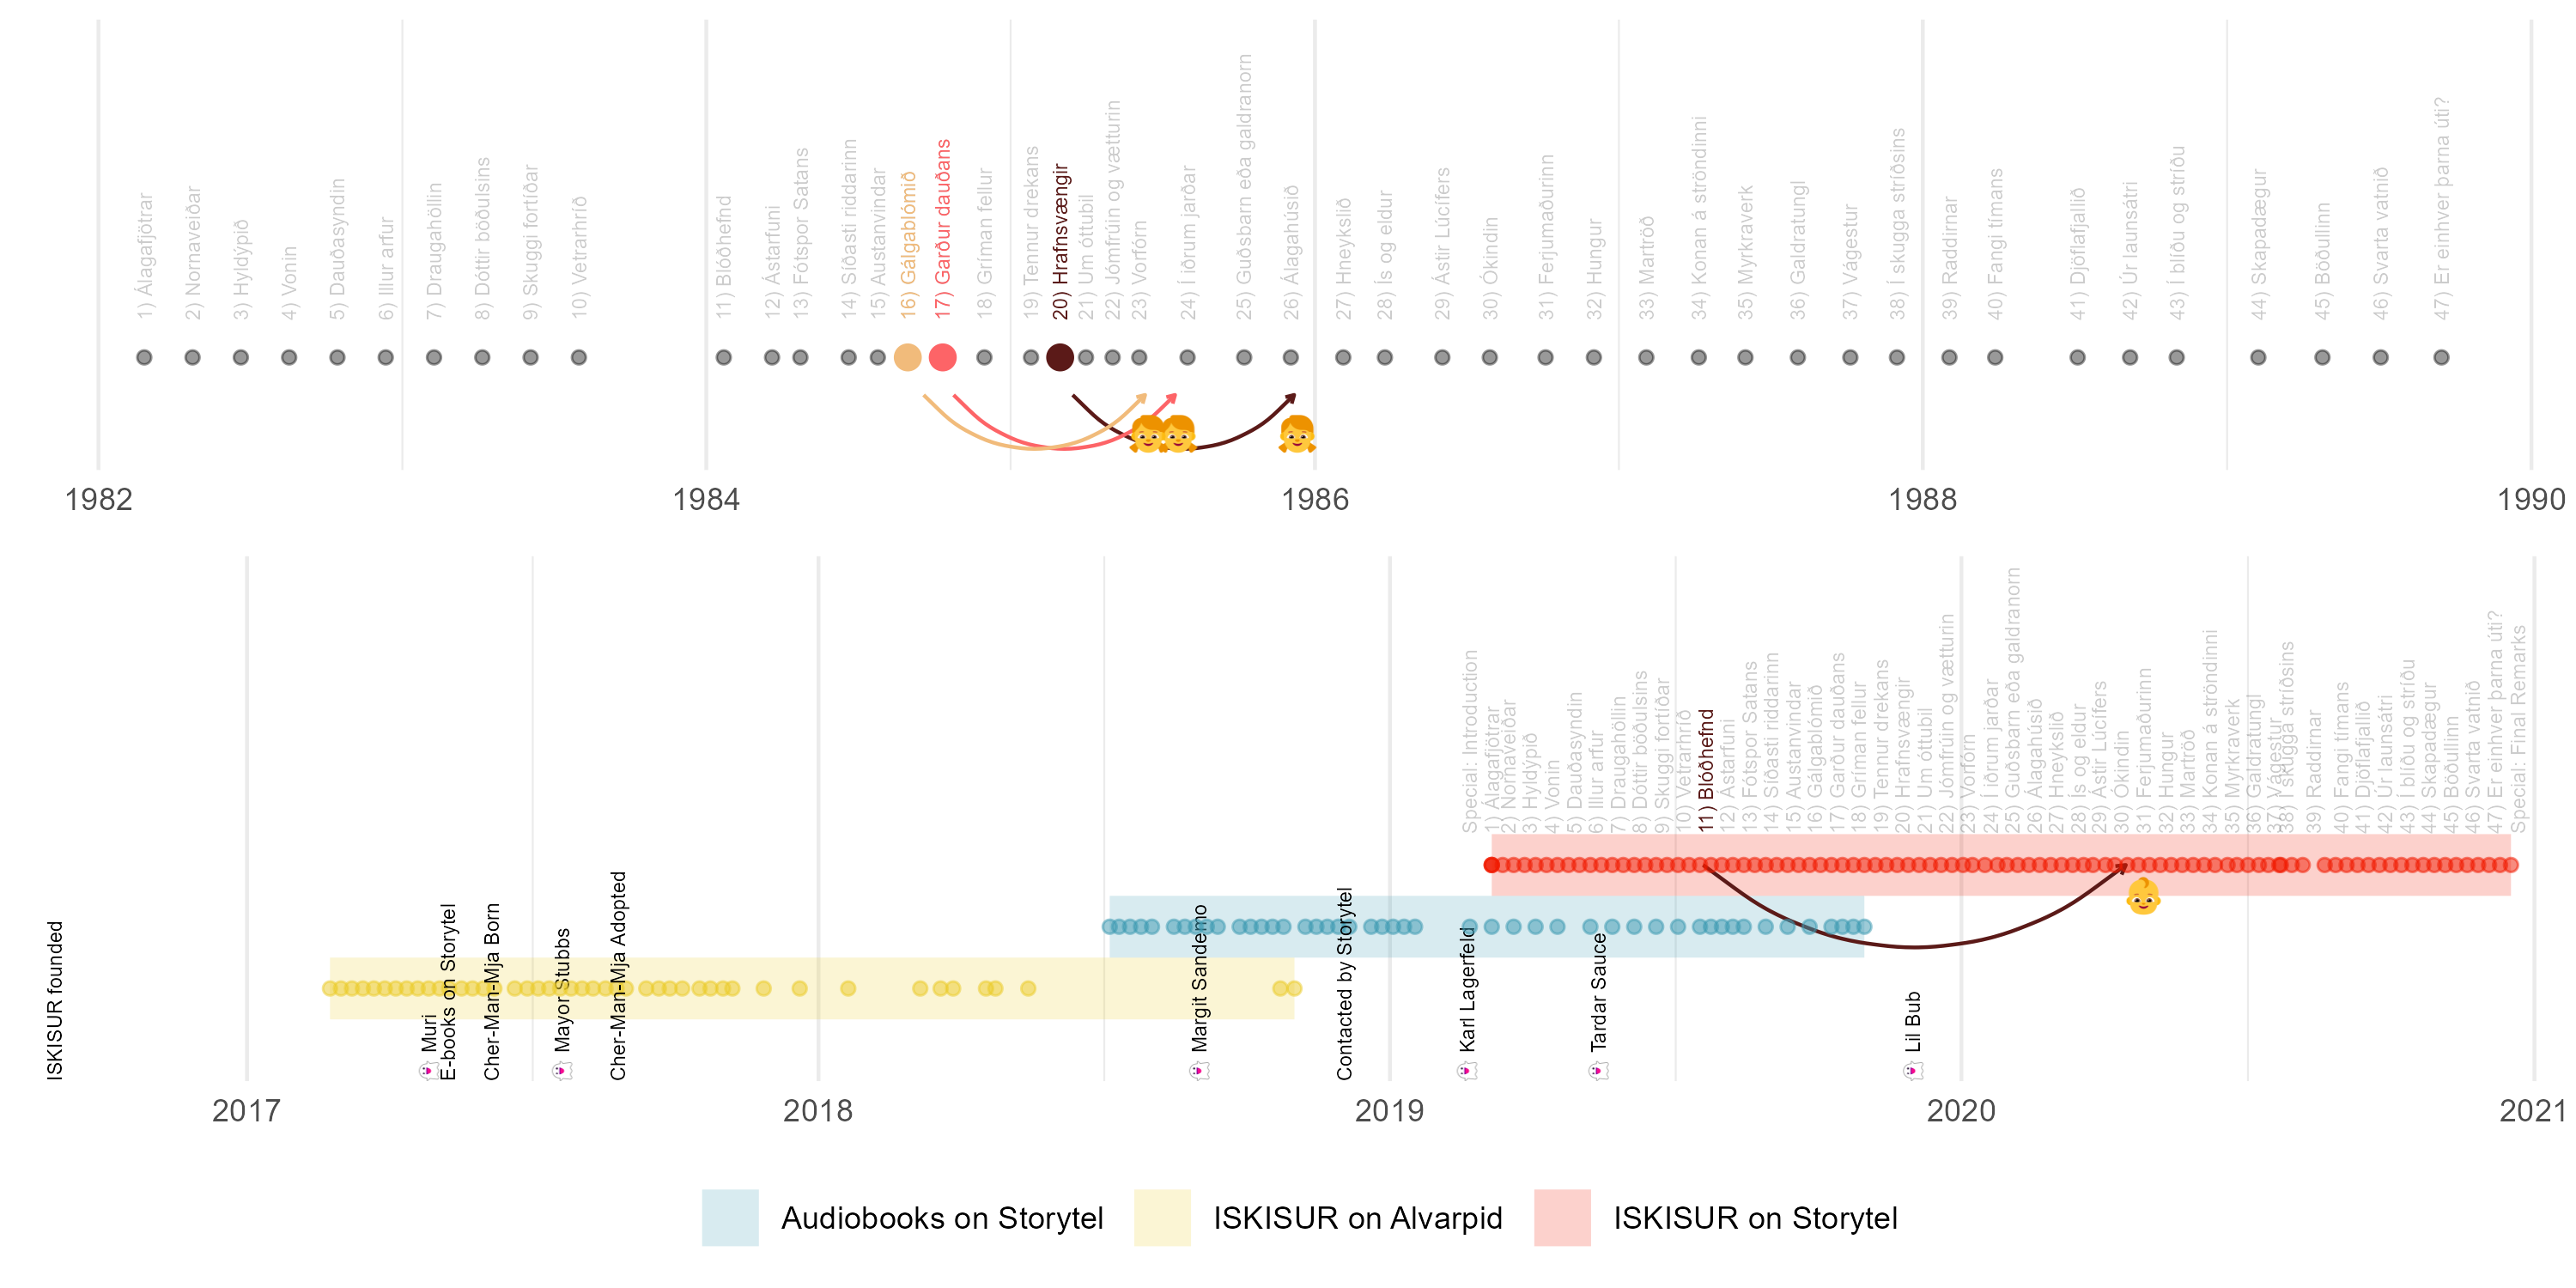
\includegraphics[width=\textwidth]{charts/timeline}
    \end{frame}

    \begin{frame}
        \frametitle{Lifespan of the Legend of the Ice People}
        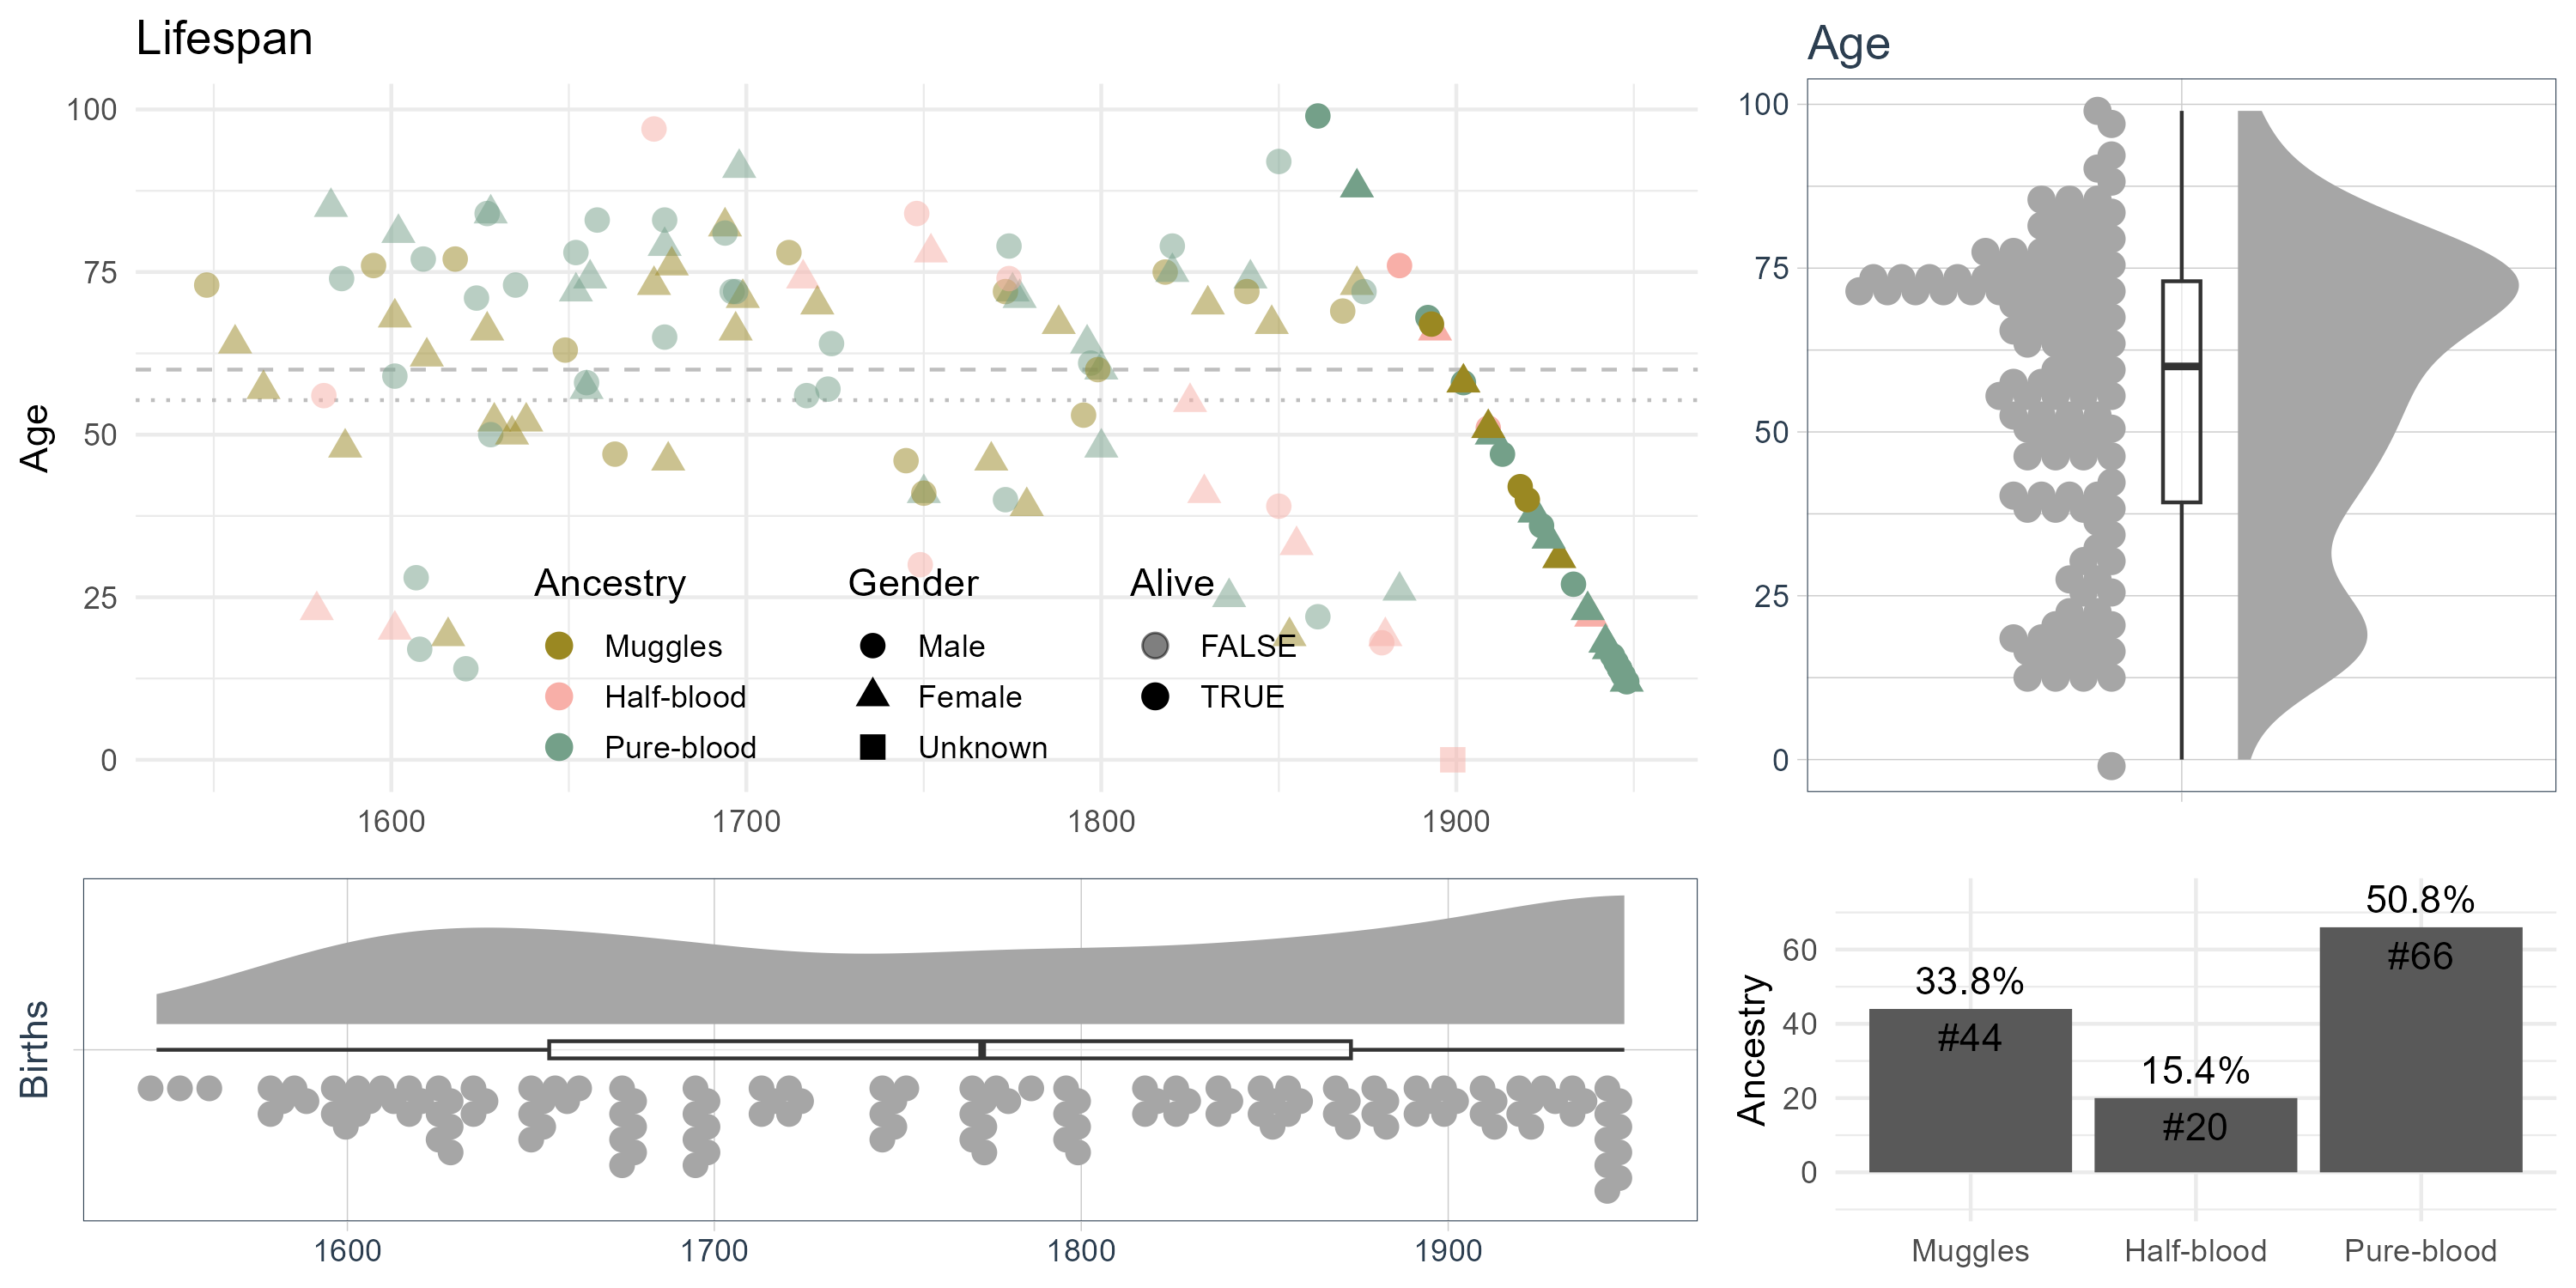
\includegraphics[width=\textwidth]{charts/family_birth}

    \end{frame}

    \begin{frame}
        \frametitle{Parental Age at Birth and Spouce Age Difference}
        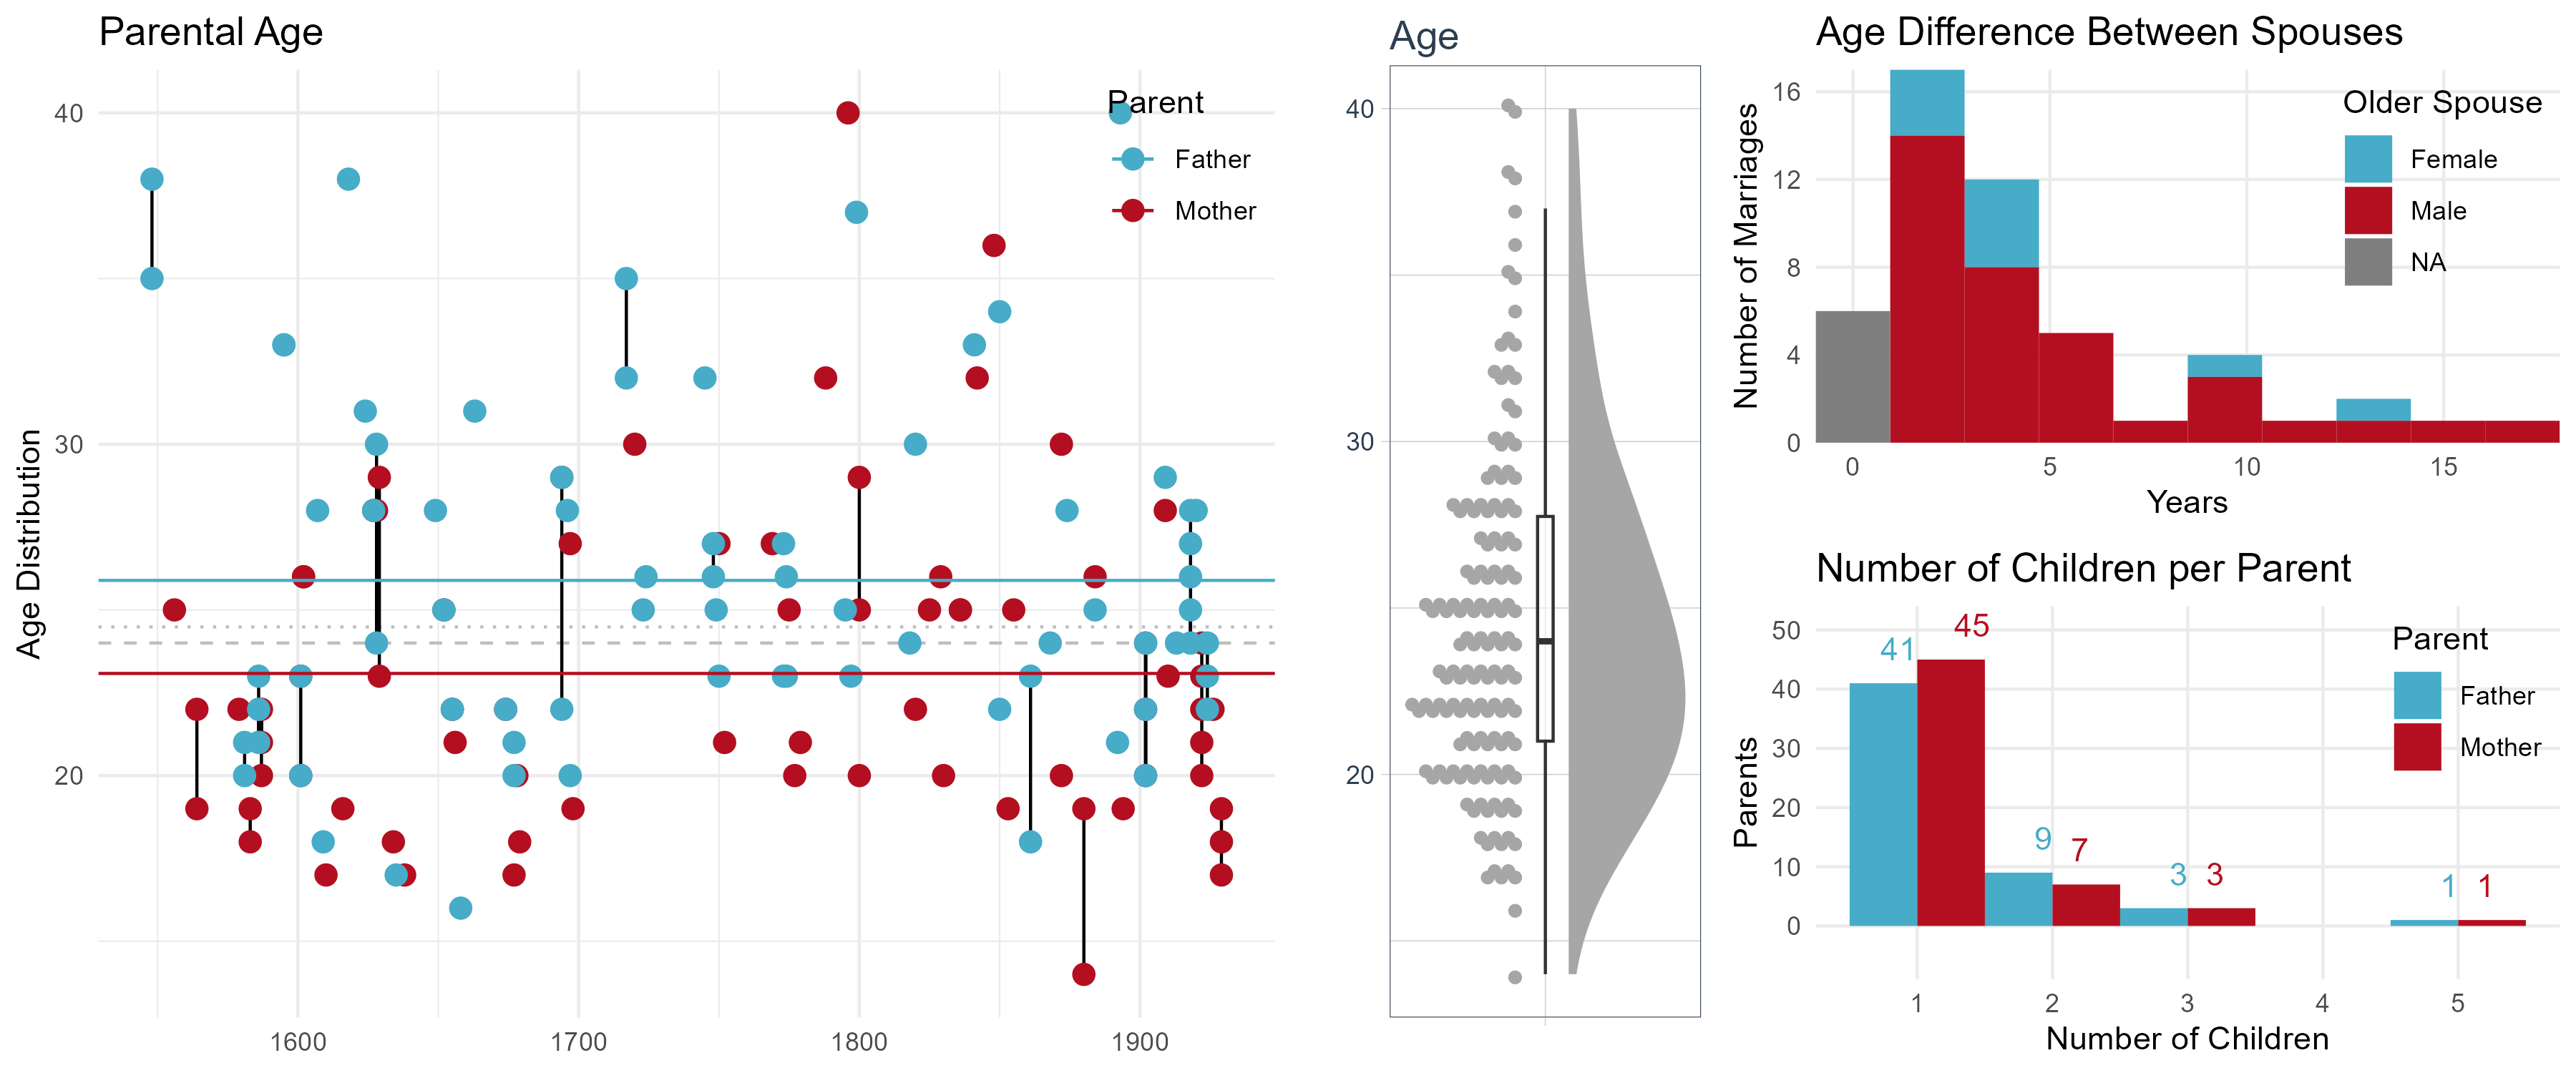
\includegraphics[width=\textwidth]{charts/family_parent_age}

        \begin{itemize}
            \item 53 relationships described, 66 children born
            \item 85\% of marriages have an older husband, age difference generally 3 years (max 17 years)
            \item Average age of mother at childbirth is 23.5 years (fathers 26.0)
            \item 22 kids have either no father (\#10) or no mother (\#12)
        \end{itemize}


    \end{frame}

    \begin{frame}
        \frametitle{Family Tree}
        \centering
        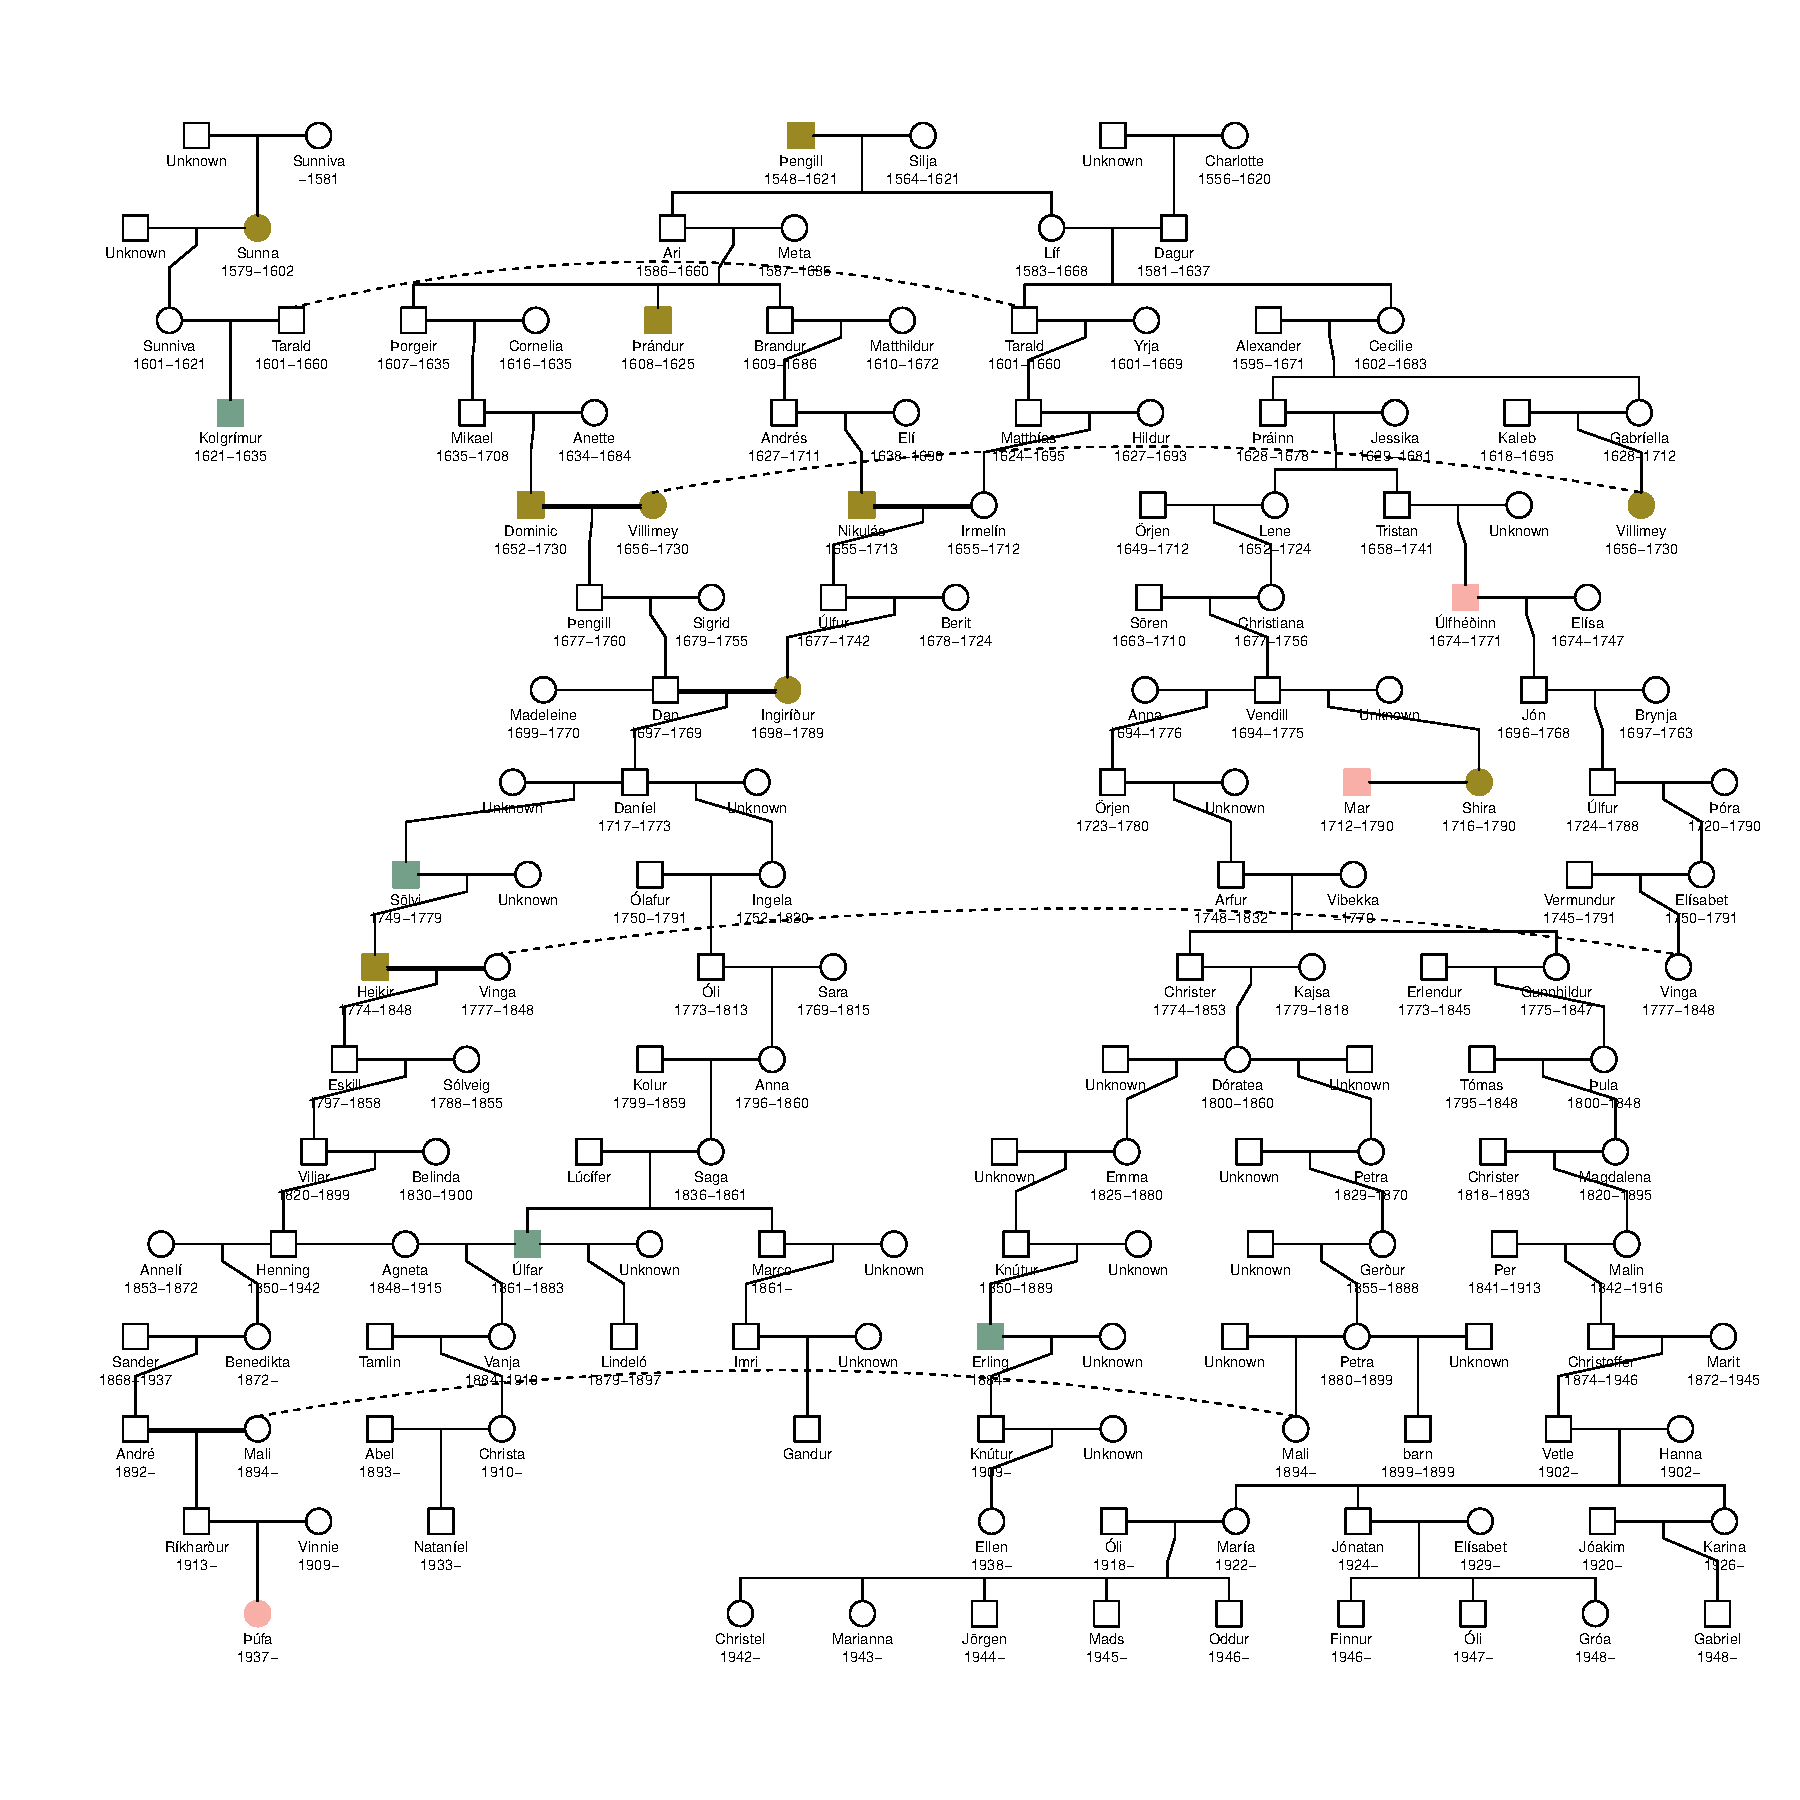
\includegraphics[height=\textheight]{charts/family_tree}
    \end{frame}

    \begin{frame}
        \frametitle{Family Gantt Chart}
        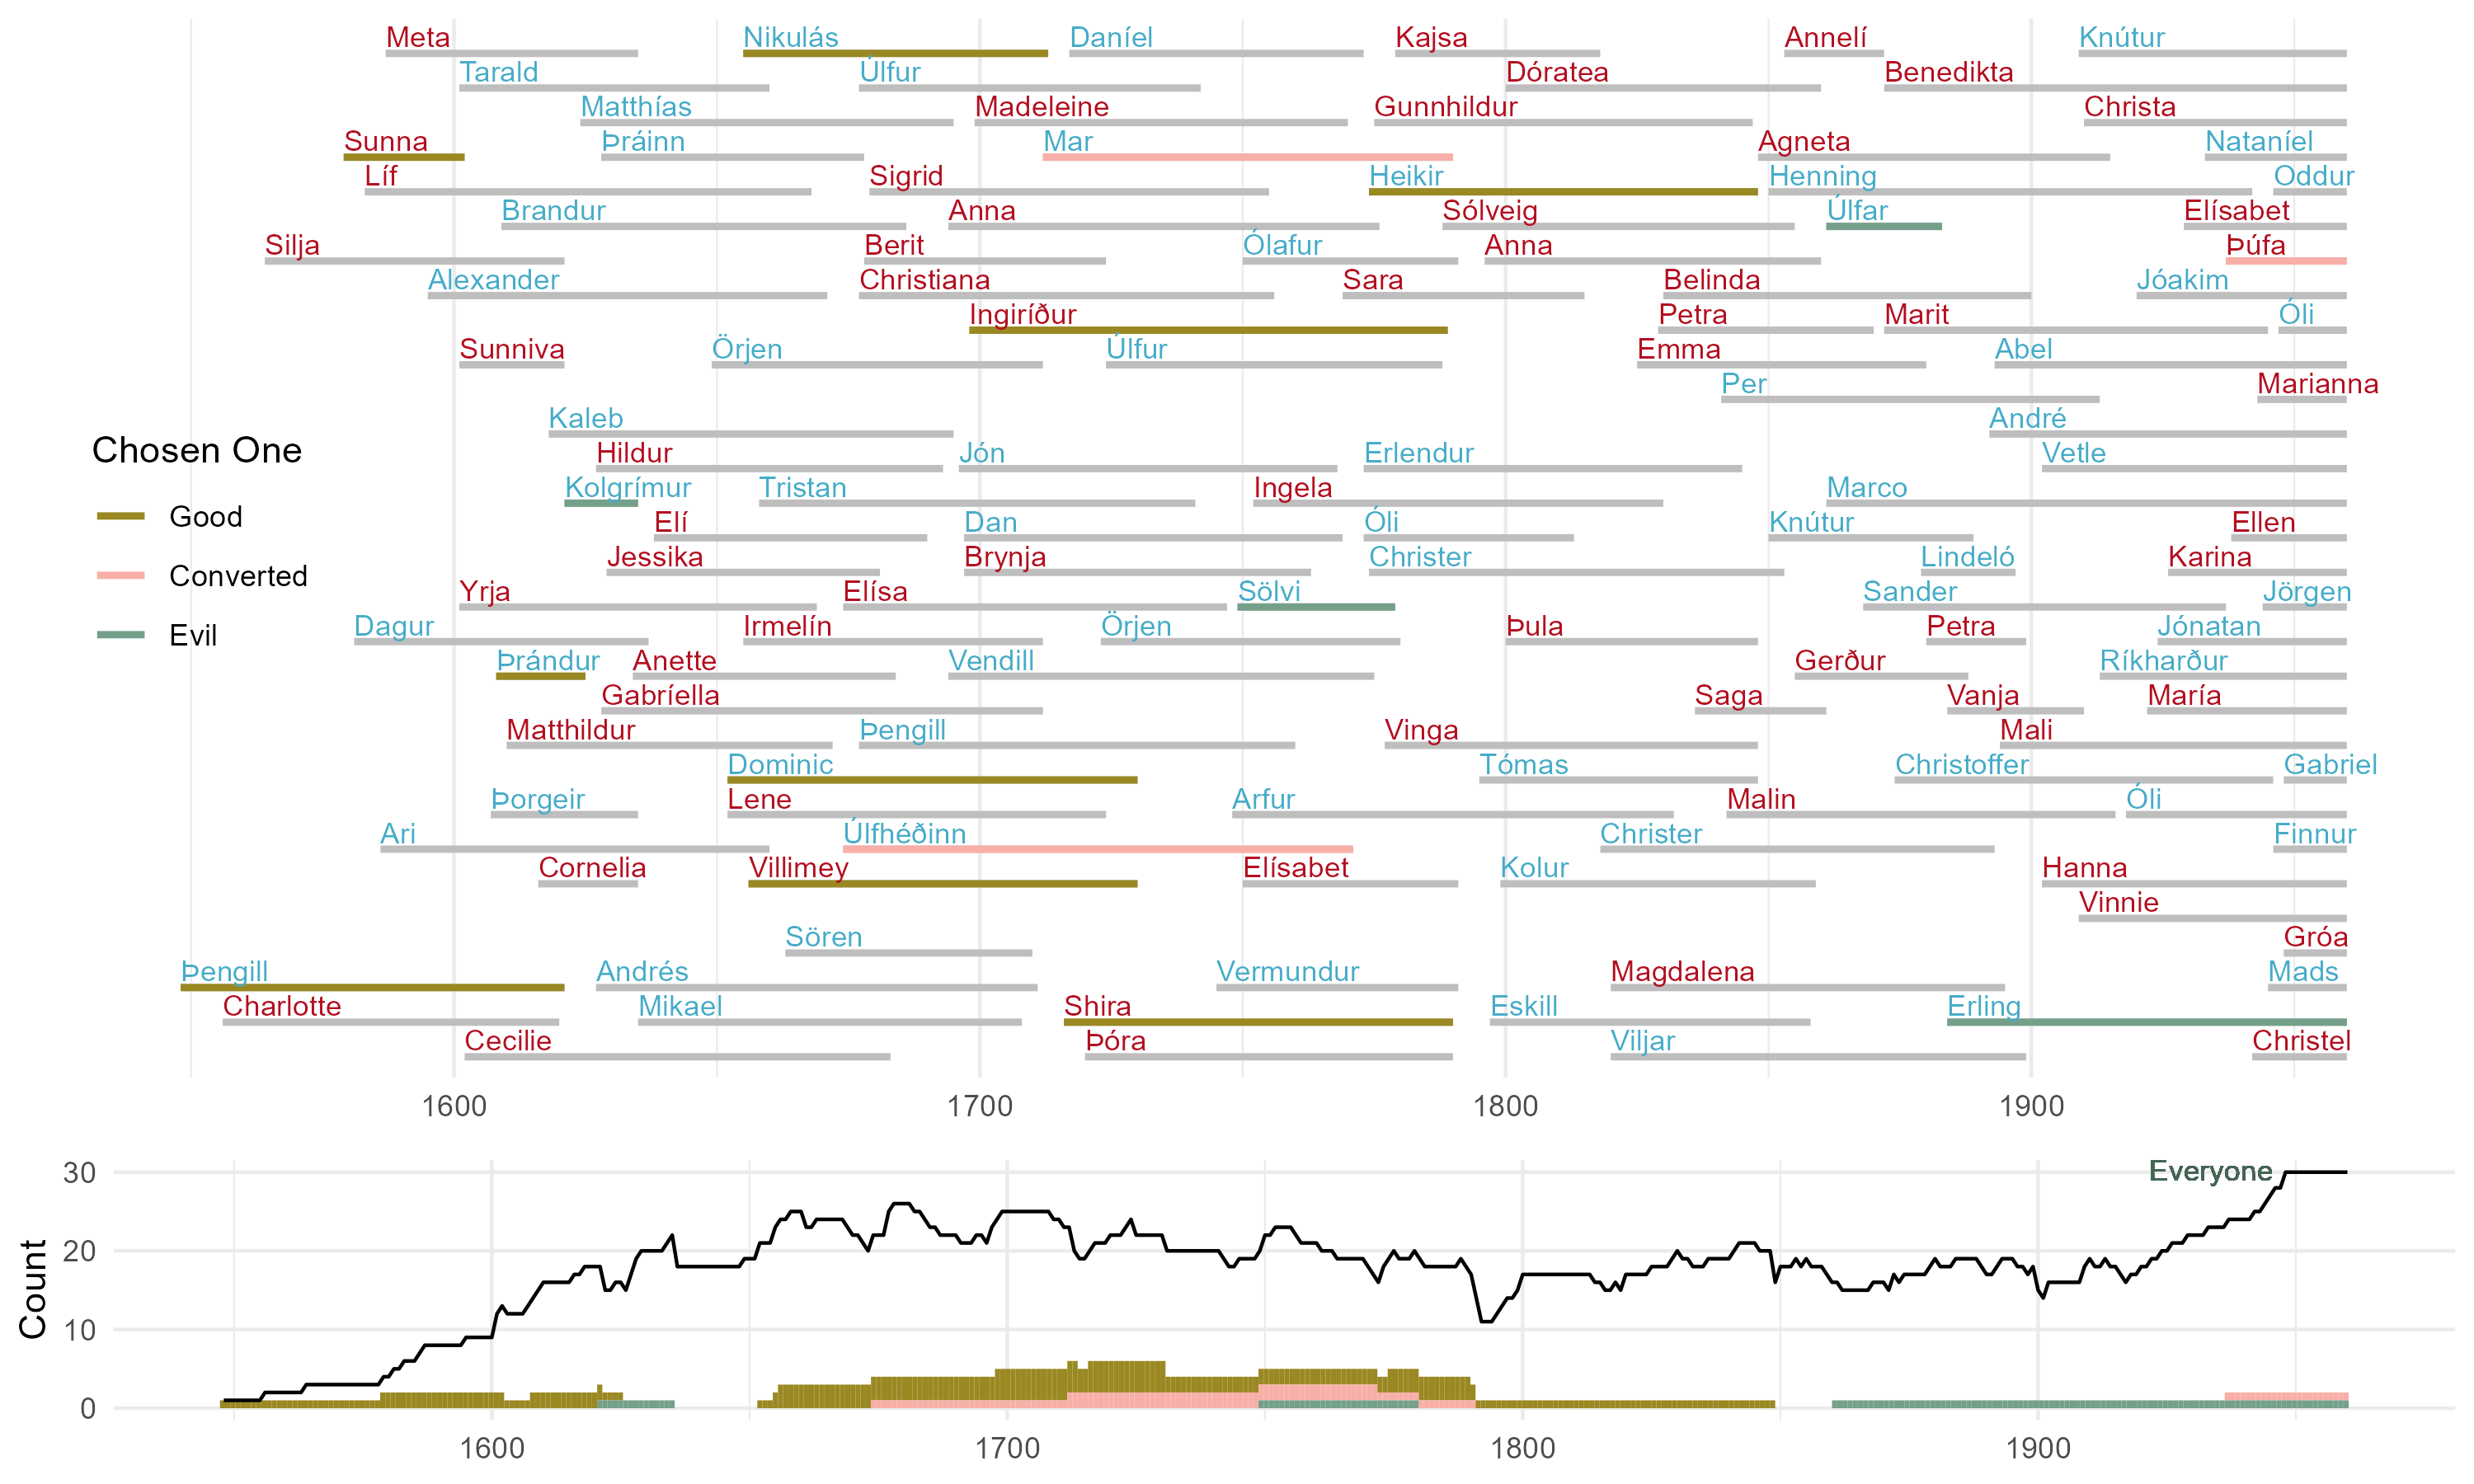
\includegraphics[width=\textwidth]{charts/family_gantt}
    \end{frame}


    \begin{frame}

    \end{frame}

    \begin{frame}
        \frametitle{Thank you!}
        Feel free to contact me at @tungufoss on Twitter and listen to the podcast on Storytel, albeit only available
        in Icelandic.

        \vspace{24pt}
        \includegraphics[width=\linewidth]{figures/iskisur_banner}

    \end{frame}

\end{document}
